Die hier besprochenen Grundlagen gehen nicht in eine Tiefe, um alle evtl. Fragen zu klären. Jedes einzelne Gebiet könnte eine Arbeit füllen. Stattdessen soll hier lediglich ein kleiner Einblick geben werden.

\section{Künstliche Intelligenz}
Die Grafik \ref{img:classification_of_terms} soll die Einordnung der besprochenen Begriffe im Bereich der Künstlichen Intelligenz (\acrshort{KI}) zeigen.

\begin{figure}[!ht]
	\includegraphics[width=0.8\textwidth]{content/chapter_basics/images/einordnung_bezeichnungen.eps}
	\centering
	\caption{Large Language Models im Kontext von Künstlicher Intelligenz}
	\label{img:classification_of_terms}
\end{figure}

In den folgenden Kapiteln werden die wichtigsten Begriffe und Technologien erläutert.\vspace{0.2cm}

Eine explizite Definition für \textit{künstliche Intelligenz} ist zurzeit noch nicht einheitlich erfolgt. Geschuldet ist diese Tatsache, dass der Begriff \textit{Intelligenz} nicht eindeutig definiert ist. Somit finden sich viele Versuche eine Definition für künstliche Intelligenz herzuleiten. Ein Ansatz Intelligenz zu erklären und definieren kommt von Jean Piaget\footnote{Jean Piaget war ein Schweizer Biologe und Pionier der kognitiven Entwicklungspsychologie. Er lebte von 9.Aug. 1896 bis 16. Sep. 1980}, welche in dieser Arbeit verwendet wird,

\epigraph[
author={Jean Piaget},
text indent=0.5cm,
after skip=0.0cm
]{Intelligenz ist ein Zustand der Balance oder des Gleichgewichts, der durch eine Person erreicht wird, wenn sie dazu fähig ist, angemessen mit den ihr vorliegenden Daten umzugehen. Aber sie [d.h. Intelligenz] ist kein statischer Zustand, sondern in dem Sinne dynamisch, dass sie sich selbst kontinuierlich an neue Umweltreize anpasst}

In dieser Arbeit wird als Definition für die Künstliche Intelligenz, die Definition aus \cite[6 ff.]{definition_ki2019} verwendet.

\epigraph[text indent=0.5cm]{
	Systeme der künstlichen Intelligenz (KI-Systeme) sind vom Menschen entwickelte Softwaresysteme (und gegebenenfalls auch Hardwaresysteme), die in Bezug auf ein komplexes Ziel auf physischer oder digitaler Ebene handeln, indem sie ihre Umgebung durch Datenerfassung wahrnehmen, die gesammelten strukturierten oder unstrukturierten Daten interpretieren, Schlussfolgerungen daraus ziehen oder die aus diesen Daten abgeleiteten Informationen verarbeiten, und über das bestmögliche Handeln zur Erreichung des vorgegebenen Ziels entscheiden. KI-Systeme können entweder symbolische Regeln verwenden oder ein numerisches Modell erlernen, und sind auch in der Lage, die Auswirkungen ihrer früheren Handlungen auf die Umgebung zu analysieren und ihr Verhalten entsprechend anzupassen.
}

%(\href{https://www.bitkom.org/sites/main/files/file/import/171012-KI-Gipfelpapier-online.pdf}{Wirtschaftliche Bedeutung ...}, 26 ff.).

\subsection{Historisches}
% aus: https://www.perplexity.ai/page/a-historical-overview-of-ai-wi-A8daV1D9Qr2STQ6tgLEOtg

An dieser Stelle eine kleine historische Exkursion in der Entwicklung der künstlichen Intelligenz.\vspace{0.2cm}

\begin{figure}[!ht]
	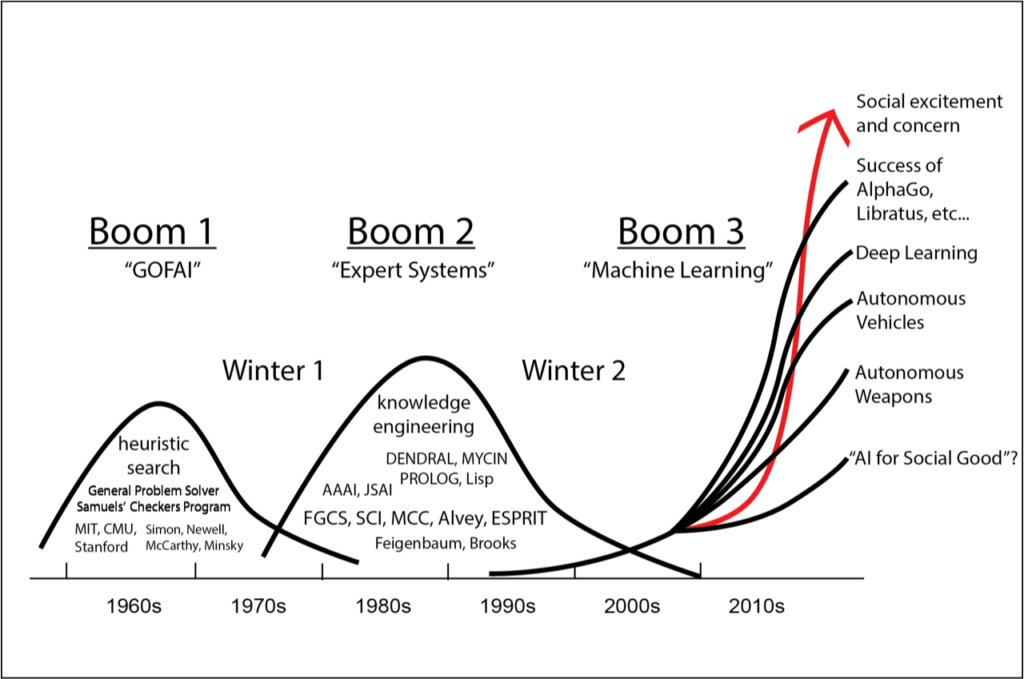
\includegraphics[width=0.8\textwidth]{content/chapter_basics/images/ai-winter-cycles.jpg}
	\centering
	\caption{KI Winterzyklen}
	\label{img:ai_winter_cycles}
\end{figure}

\textbf{1966: Rückschläge bei der maschinellen Übersetzung} brachten die Entwicklung nahezu zum Erliegen, lediglich einige wenige Gruppen. Durch die Bedrohungsszenarien des \textit{Kalten Krieges} wurden von der US-Regierung und Militär Unsummen von Geldern bereitgestellt, um die Forschung von maschinellen Übersetzungen voran zutreiben. Durch die ausbleibenden Erfolge wurden diese Gelder jedoch gestrichen.\vspace{0.2cm}

Frank Rosenblatt führte 1958 das Perzeptron ein, das in der Lage war einfache logische Operationen in Neuronalen Netzen auszuführen. Ein Problem was diese Netzwerke nicht lösen konnten war die \textit{nicht lineare Trennbarkeit}, wie beispielsweise das XOR-Problem. Dieses Problem wurde in der Arbeit von Marvin Minskys und Seymour Papert gezeigt. Diese Arbeit beeinflusste die Entwicklung so massiv, dass \textbf{1969: die Auswirkungen der Perzeptron-Kritik} dazu betrugen den ersten KI-Winter auszulösen.\vspace{0.2cm}

\textbf{1971-75: Die Finanzierungskürzung der DARPA (Defense Advanced Research Projects Agency)}, die aufgrund der Unzufriedenheit, bei den Fortschritten natürliche Sprache in realen Szenarien, effektiv durch Systeme verarbeiten zu können, trug ebenfalls zur Auslösung des ersten KI-Winters bei. Diese Entscheidung übertrug sich auch auf andere Bereiche in der KI Entwicklung.\vspace{0.2cm}

\textbf{1973: Der Fallout des Lighthill-Berichts} war der entscheidende Faktor, das den KI-Winter auslöste. Dieser Bericht bewertet die wies auf erhebliche Mängel in den Bereichen Robotik und Sprachverarbeitung hin. Der Bericht führte zu einer erheblichen Skepsis gegenüber der KI und in vielen Projekten zur Kürzung der Fördermittel. Er wirkte sich auch auf die Moral und das Vertrauen der Community aus, welche aus diesem Grund nur sehr kleine und vorsichtige Fortschritte in der KI Forschung erzielte.\vspace{0.2cm}

Der \textbf{1987: Zusammenbruch der LISP-Maschine} markierte den Beginn des \textit{zweiten KI-Winters}. Die spezialisierten LISP-Maschinen, erfuhren einen Nachfragerückgang, ausgelöst durch neu entwickelten Allzweckcomputer von IBM und Apple. Dieses Ereignis zeigt auch beispielhaft wie technologische und wirtschaftliche Faktoren zur Neubewertung und Neuausrichtung ganzer Fachrichtungen führen können.\vspace{0.2cm}

Die \textbf{1988: Strategischen Kürzungen im Computerbereich} durch die US-Regierung trugen ebenfalls zum Ausbruch des \textit{zweiten KI-Winters} bei. Auslöser waren die enttäuschenden Ergebnisse und unerfüllten Erwartungen der Forschung in verschiedenen KI Projekten. Dadurch erfolgte eine Neubewertung der Investitionspriorisierung und führte zu einer deutlichen Kürzung der Gelder. Diese Bewertung wirkte sich auch auf viele weitere Projekte der KI-Entwicklung aus, sodass diese ganz aufgegeben und neue Technologien erforscht und entwickelt wurden.\vspace{0.2cm}

In den \textbf{1990er Jahre: war der Niedergang von Expertensystemen} ebenfalls ein Auslöser, der dazu betrug, dass die Entwicklung von KI-Systemen stagnierte. Deren Wartung war sehr kosten- und arbeitsintensiv, ebenfalls wurden die ständig aktuell benötigten Datenbanken nicht automatisiert aktualisiert. Auch erfüllten sie nicht die in ihnen gesetzten Erwartungen. \vspace{0.2cm}

In den Jahren nach 2000 bis 2020 trat ein bedeutender Wandel bei den KI-Technologien ein, der als \textbf{KI-Frühling des frühen 21. Jahrhunderts} gesehen wird. Besonders die Fortschritte im Bereich \textit{maschinelles Lernen}, \textit{Deep Learning}, und \textit{neuronale Netze} sorgten für neue Investitionen in diesen Bereichen. Besonders namhafte Tech-Firmen, wie IBM, Google und Microsoft stellten große Budges für die Forschung. Gefördert wurde die Entwicklung durch neue leistungsfähigere Rechner und Daten die in großen Mengen zur Verfügung standen. Hinzu kam, dass KI in die Mainstream-Technologie integriert und in viele Geschäftsprozesse Einzug hielt.\vspace{0.2cm}


\subsection{Maschinelles Lernen}
Das Gebiet um das Maschinelle Lernen (\acrshort{ML}) ist ein Teilgebiet der Künstlichen Intelligenz. Für das maschinelle Lernen wird in dieser Arbeit die allgemein gültige Definition nach Tom M. Mitchell verwendet.\vspace{0.2cm}

\epigraph[
author={Mitchell, Tom M},
source={Machine Learning},
translation={Ein Computerprogramm lernt aus Erfahrung E in Bezug auf eine Klasse von Aufgaben T und ein Leistungsmaß P, wenn sich seine Leistung bei Aufgaben in T, gemessen an P, mit der Erfahrung E verbessert.}
]{
	A computer programm is said to learn from experience E with respekt to some class of tasks T and performance measure P, if its performance at tasks in T, as measured by P, improves with experience E.
}

Bei dieser Definition ist,\\
\textbf{E} die \textbf{Erfahrung}, die Daten aus denen das System lernt,\\
\textbf{T} beschreibt die \textbf{Aufgabe}, die das System erledigen soll und\\
\textbf{P} ist die \textbf{Leistungskennzahl} an dem der Erfolg des Systems die Aufgabe zu lösen gemessen wird.\vspace{0.2cm}
%Da es mehrere Definitionen maschinellen Lernens gibt definieren WITTEN ET AL. (2001:6) eine operationale Definition von Lernen: „Etwas lernt, wenn es sein Verhalten so ändert, dass es in Zukunft eine bessere Leistung aufweist.“

\acrshort{ML} und \acrshort{KI} sind nicht wirklich in der Lage selbstständig zu lernen oder denken, sie imitieren dies lediglich. \acrshort{ML} ist aber wohl in der Lage komplexe Muster und Funktionen in großen Datenmengen zu erkennen. Durch die Unfähigkeit zu lernen sind KI Technologie nicht in der Lage neuen Inhalte zu schaffen.\vspace{0.2cm}

Es ist auch egal wie gut die Modelle trainiert werden, eine 100\% Fehlerfreiheit gibt es nicht. Für die Praxis bedeutet dies, die Ausgaben von Modellen müssen durch Menschen immer wieder evaluiert werden, um dessen Richtigkeit sicherzustellen. Zudem sollten keine Modelle verwendet werden, wenn die Lösung eines Problems durch einen konkreten Algorithmus erfolgen kann. Hier können die Ergebnisse nachvollzogen werden und sind für den Menschen besser zu verstehen.\vspace{0.2cm}

\begin{figure}[!ht]
	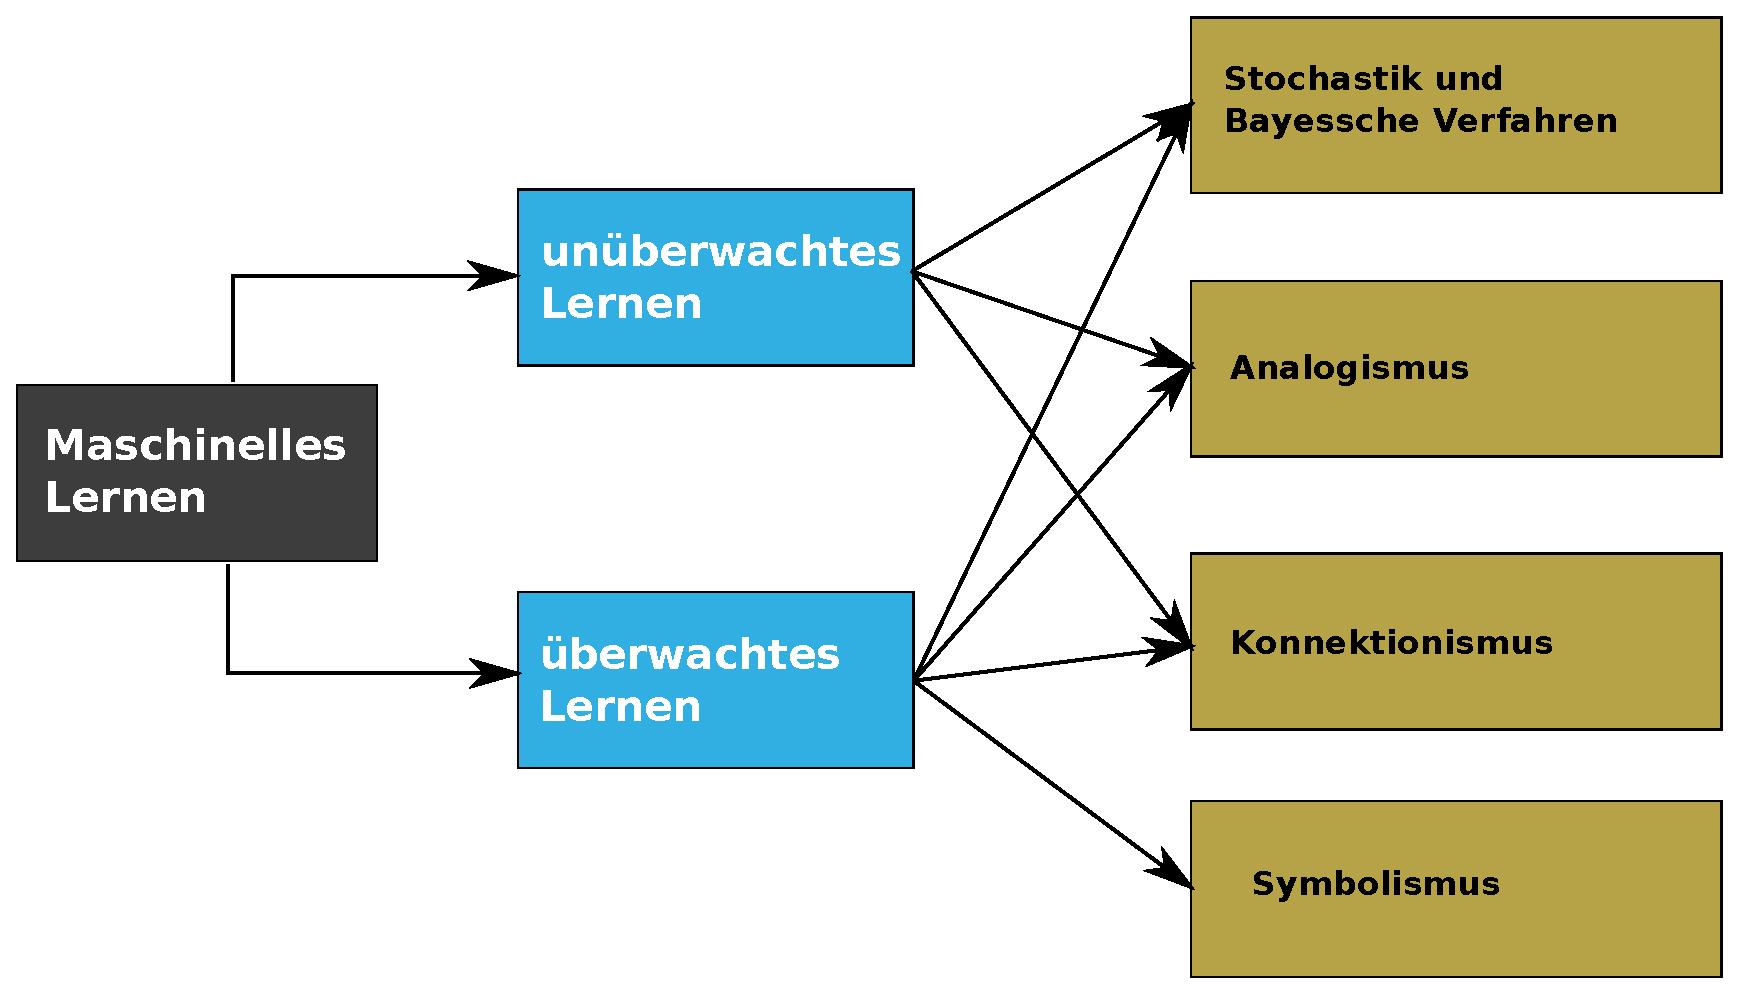
\includegraphics[width=0.8\textwidth]{content/chapter_basics/images/learning_paradigmen_ml_v2.eps}
	\centering
	\caption{Lernparadigmen des maschinellen Lernens}
	\label{img:learning_paradigms_of_ml}
\end{figure}


\subsection{Lernparadigmen des ML}
Das maschinelle Lernen wird in zwei wichtige Formen der Lernparadigmen unterteilt. Dem überwachten (supervised Learning) und unüberwachten Lernen (unsupervised Learning). Abbildung \ref{img:learning_paradigms_of_ml} zeigt die wichtigsten Lernparadigmen des maschinellen Lernens und dessen Methodiken.

\subsubsection{Überwachtes Lernen}
Bei überwachten Lernen sind für die Eingaben der Trainingsdaten dazugehörige Ausgaben (Labels) definiert. Das Ziel ist es eine Funktion zu trainieren um künftige Eingaben korrekt klassifizieren oder vorhersagen zu können.

\subsubsection{Unüberwachtes Lernen}
Bei unüberwachten Lernen sind die gelabelten Ausgaben nicht vorhanden. Hierbei wird beispielsweise durch Clustering oder Dimensionsreduktion versucht Muster und Strukturen zu erkennen.


\subsection{Theoretische Grundlagen des Lernens}
In den folgenden Kapiteln werden vier wichtige Konzepte zum maschinellen Lernen besprochen. 

\subsubsection{Stochastik und Bayessches Theorem}
Als Teilgebiet der Mathematik befasst sich die Stochastik mit Wahrscheinlichkeitsverteilung und zufälligen Prozessen. Auf dem Gebiet des maschinellen Lernens werden mithilfe der Stochastik Prognosen erstellt. Es wird versucht auf der Basis vorhandener Daten, bei neuen Daten eine Wahrscheinlichkeitsverteilung vorherzusagen. Durch geeignete Modellierung wird versucht einen kontrollierten Umgang mit Unsicherheiten zu erlangen.\vspace{0.2cm}

Bei den Bayesschen Theorem handelt es sich um stochastische Methoden, die auf dem Bayessches Theorem basieren. Mit dessen Hilfe soll auf Basis der vorliegenden Daten das beste Modell, für die Vorhersage gefunden werden. Das Verfahren berücksichtigt immer die neusten Daten, um die Wahrscheinlichkeitsverteilung zu aktualisieren. Siehe Formel \ref{eq:bayessches_theorem}

\xequation{Bayessches Theorme}{
	\label{eq:bayessches_theorem}
	P(A|B) = \frac{P(B|A) \cdot P(A)}{P(B)}
}

%Beide Methoden finden im überwachten und unüberwachtes Lernen Anwendung.

\subsubsection{Analogismus}
Dieser Lernansatz sucht nach Ähnlichkeiten in den Daten. Er basiert auf der Annahme, dass ähnliche Daten ähnliche Vorhersagen oder Klassifizierungen besitzen. Dieses Modell lernt, indem neue Daten mit bekannten vergleicht und nach ähnlichen Strukturen und Mustern sucht. Ein bekanntes Verfahren für diesen Lernansatz ist der k-Nearest Neighbors (\acrshort{k-NN}).\vspace{0.2cm}

Der Analogismus wird im überwachten Lernen als auch im unüberwachten Lernen angewandt, um Muster und Strukturen zuerkennen.

\subsubsection{Konnektionismus}
Der Lernansatz des Konnektionismus beruht auf kleine Einheiten die miteinander verbunden sind. Diese werden als Neuronen bezeichnet, die den Nervenzellen von Organismen nachempfunden sind. Die Künstlichen neuronalen Netze sind die bekanntesten Vertreter auf denen auch Deep Learning Modelle basieren.\vspace{0.2cm}

Auch dieser Lernansatz wird im unüberwachten und überwachten Lernen angewandt.

\subsubsection{Symbolismus}
Anders als beim Konnektionismus arbeiten die Einheiten beim Symbolismus mit explizite formale Regeln und Symbole, um das Wissen darzustellen. Der Symbolismus ist weniger flexible im Umgang mit unvollständigen Datensätzen und Unsicherheiten. Daher hat dieser Lernansatz weniger Relevanz als der Konnektionismus.\vspace{0.2cm}

Dieser Lernansatz findet im überwachten Lernen Anwendung, als Beispiel sind hier Entscheidungsbäume zu nennen.

% --- LOS ----------------------------


\subsection{Neuronale Netze}
Neuronale Netze oder auch künstliche neuronale Netze (\acrshort{KNN}) sind spezifische Typen des maschinellen Lernens. Sie sollen die biologischen Neuronen des Gehirns nachempfinden. Die Abbildung \ref{img:biological_neuron} von \cite{pahl-2024} zeigt eine stark vereinfachte biologische Nervenzelle.

\begin{figure}[!ht]
	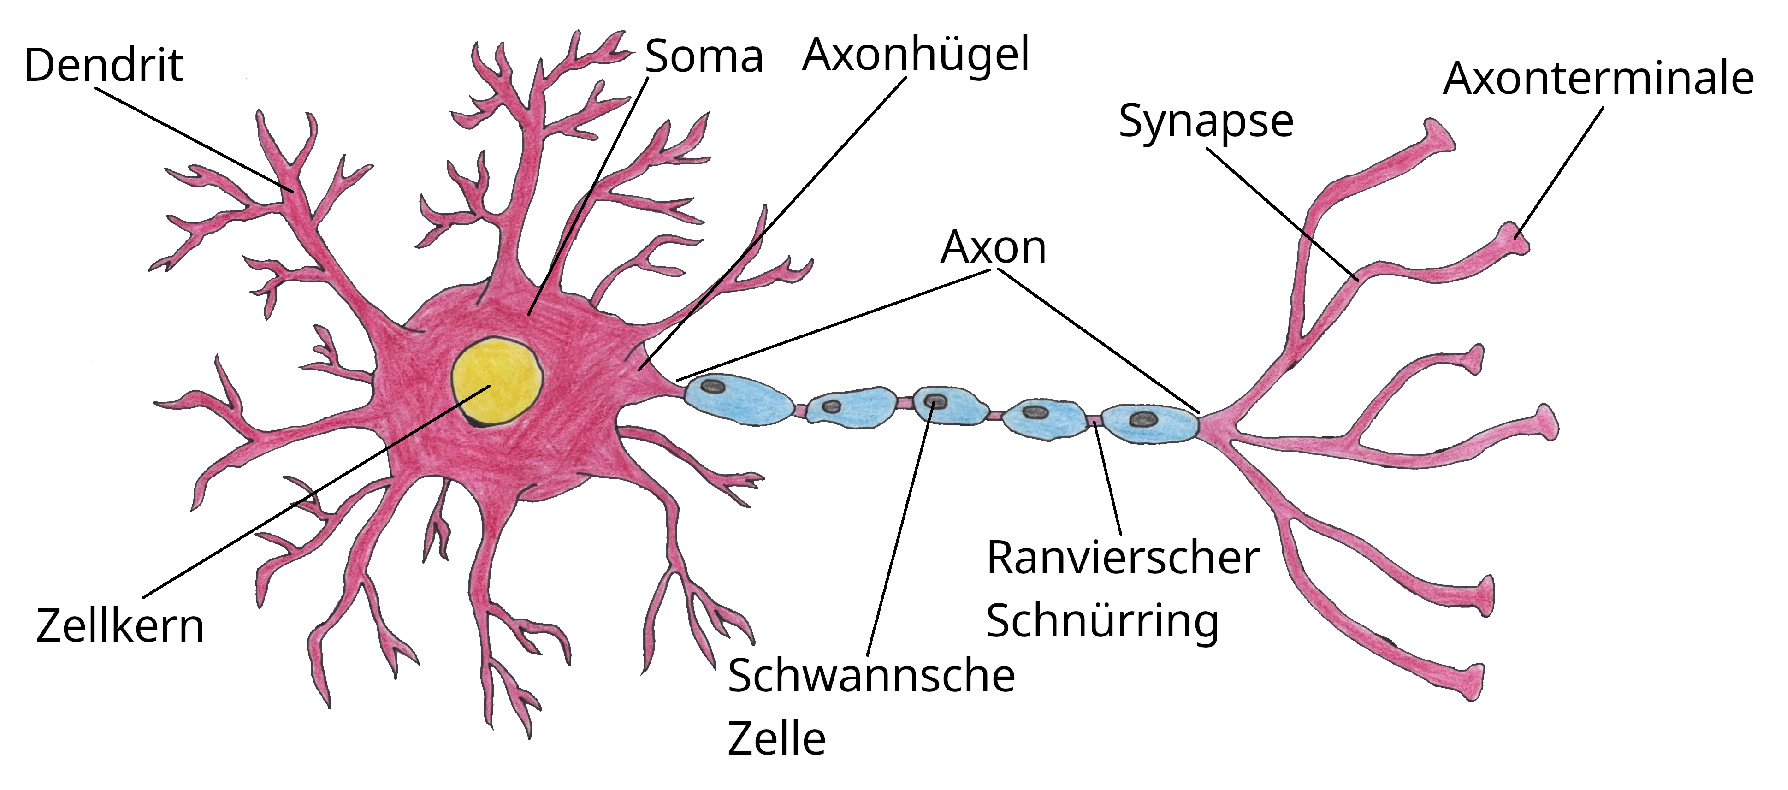
\includegraphics[width=0.8\textwidth]{content/chapter_basics/images/biological_neuron.eps}
	\centering
	\caption{Biologische Nervenzelle}
	\label{img:biological_neuron}
\end{figure}

Bei Nervenzellen werden elektrische Eingangssignale über Dendriten aufgenommen und in den Zellkern geleitet. Dort werden die eingehenden Signale zusammen geführt und es bildet sich das Aktionspotential. Übersteigt das Aktionspotential das Schwellenpotential der Zelle, so wird das Signal über das Axon abgeleitet, die Nervenzelle \glqq \textit{feuert}\grqq.\vspace{0.2cm}

Bevor das Signal die nächste Nervenzelle reizen kann, muss es über den synaptischen Spalt. Hierbei ist die Präsynapse das Axon der sendenden Zelle, die Postsynapse ist ein Dendrit der empfangenden Nervenzelle. Der Reiz wird durch die Botenstoffe Dopamin oder Serotonin übertragen. Dopamin wirkt als Verstärker der Reizübertragung, während Serotonin hemmend wirkt.

\subsubsection{Neuronen im neuronalen Netz}
Die kleinste Einheit in künstlichen neuronalen Netzen sind die Neuronen. Sie sind den biologischen Nervenzellen nachempfunden. \vspace{0.2cm}

\begin{figure}[!ht]
	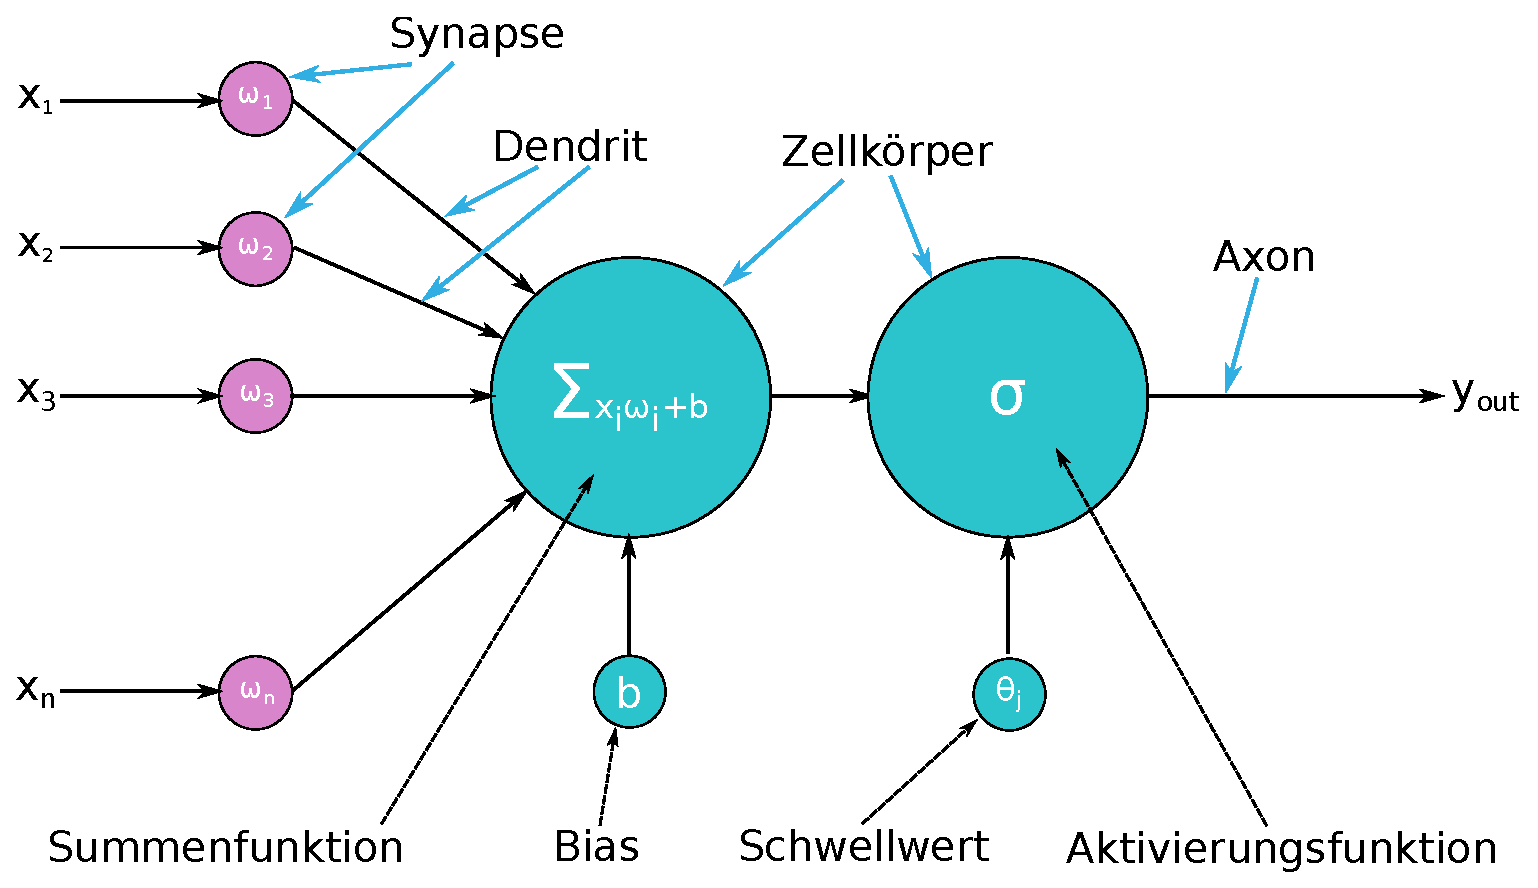
\includegraphics[width=0.8\textwidth]{content/chapter_basics/images/artificial_neuron.eps}
	\centering
	\caption{Künstliche Nervenzelle}
	\label{img:artificial_neuron}
\end{figure}

Sie haben als Eingangswert einen Vektor und als Ausgangssignal ein Skalar. Außer in der Eingabe Schicht ist jedes Eingangssignal $x_n$ ein Ausgangssignal $y_{out}$ eines anderen Neuron. Die Wichtungen der Eingangssignale modellieren den synaptischen Spalt zwischen zwei biologischen Nervenzellen. Dieser kann ebenfalls verstärkten oder hemmend wirken. Alle Eingangssignale zusammen mit den Wichtungen, werden durch die Summenfunktion aufaddiert. Im Anschluss wird das \gls{bias} mit eingerechnet. Die Formel \ref{eq:sum_function} zeigt die Summenfunktion für $n$ Eingangssignale mit Beachtung des Bias Wert.

%\begin{equation} \label{eq:sum_function}
%	y = x_{1} + x_{2} + \dots + x_{n} + b
%\end{equation}
\xequation{Summenfunktion}{
	\label{eq:sum_function}
	y = x_{1} + x_{2} + \dots + x_{n} + b
}

Durch das Bias wird die Berechnung in der Summenfunktion flexibler, eine Verschiebung in Richtung der y-Achse ist möglich, ohne die Wichtungen anzupassen und es ermöglicht eine Ausgabe auch, wenn alle Eingänge $Null$ sind.\vspace{0.2cm}

Nach der Summenfunktion wird das Signal an die Aktivierungsfunktion übergeben. Diese Funktion leitet ein Signal erst weiter, wenn ein festgelegter Schwellwert überschritten wird. Die Analogie zur biologischen Nervenzelle ist das Aktionspotential, welches durch die Reize anderer Nervenzellen aufgebaut wird und wie beim künstlichen Neuron führt das Überschreiten eines Schwellenwertes dazu, dass das Neuron \glqq feuert\grqq. \vspace{0.2cm}

% https://www.mind-verse.de/post/aktivierungsfunktionen-neuronale-netzwerke-rollen-typen

Je nach Problem ist es wichtig die richtige Aktivierungsfunktion zu wählen. In \cite{brownlee-2021} wird beschrieben wie dies erfolgen kann, hier ist die Abbildung \ref{img:selection_activation_function} entnommen.

\begin{figure}[!ht]
	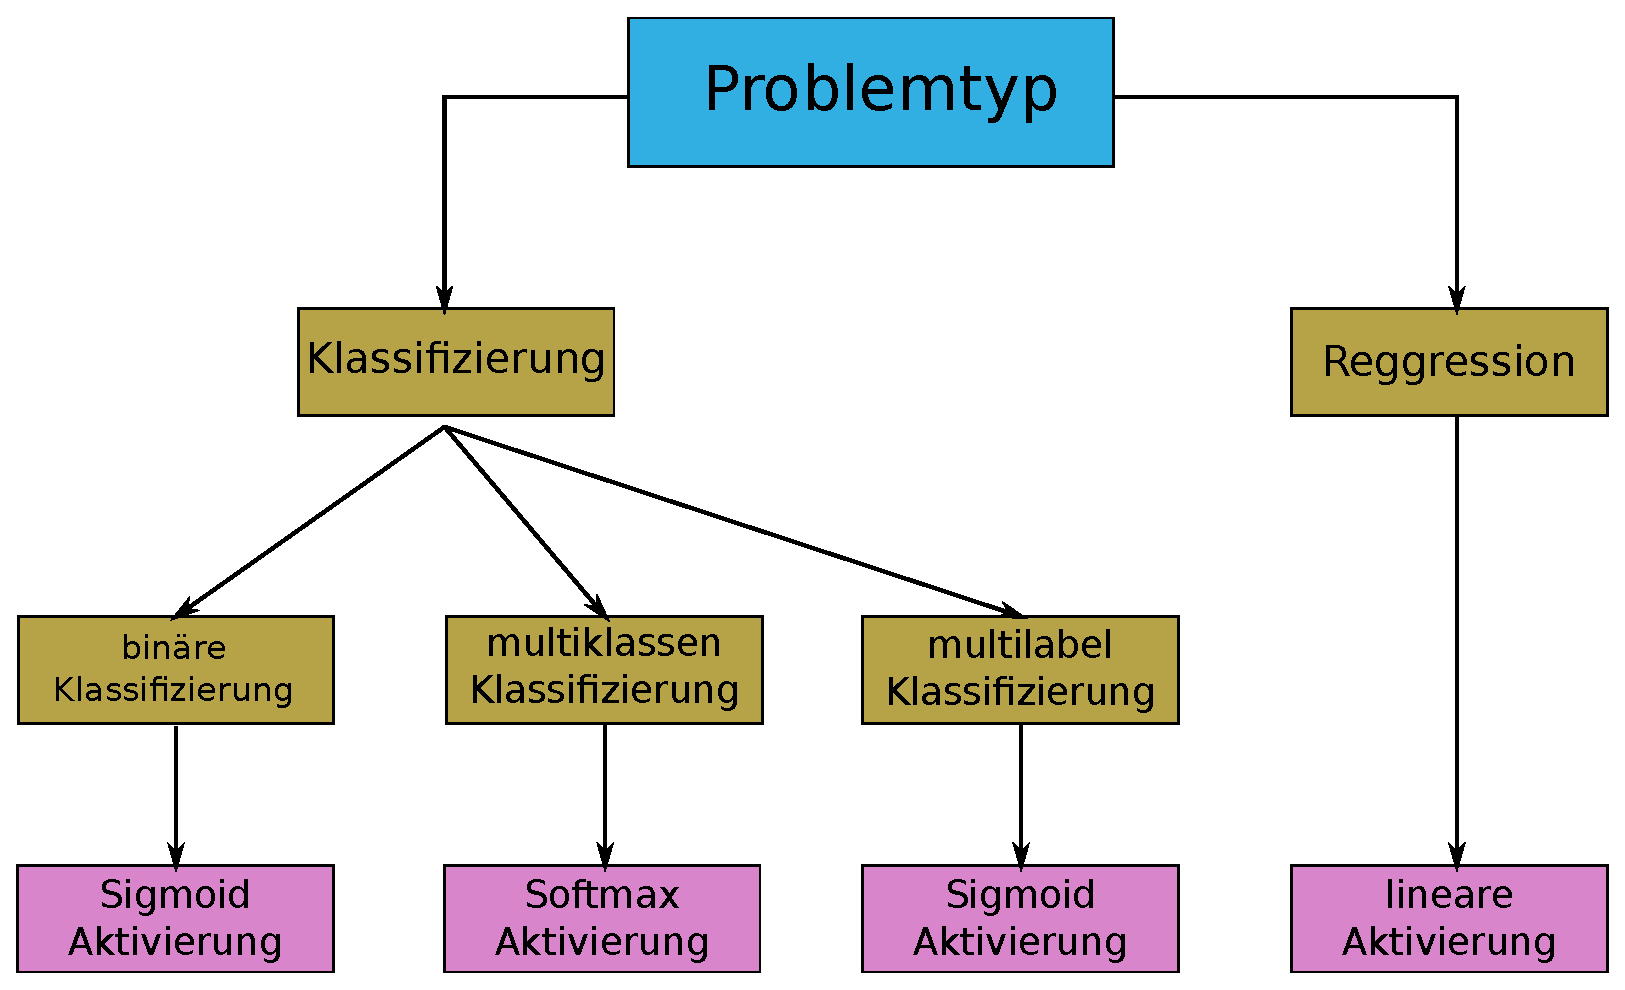
\includegraphics[width=0.8\textwidth]{content/chapter_basics/images/activation_select.eps}
	\centering
	\caption{Auswahl der richtigen Aktivierungsfunktion}
	\label{img:selection_activation_function}
\end{figure}

Im Folgenden werden einige Aktivierungsfunktionen vorgestellt.\vspace{0.2cm}

%%----------------------------------------------------------------------------
%   Identity
%
\textbf{Identity-Aktivierungsfunktion}\vspace{0.2cm}

Die Gleichung der Identity Funktion ist in Formel \ref{eq:identity_activation_function} zu sehen. Da die Ausgabe der Eingabe entspricht, sind alle Werte möglich die in der Summenfunktion entstehen. Aus ihr geht hervor das der Wertebereich theoretisch von $-\infty$ bis $\infty$ reicht.\vspace{0.2cm}

Einsatz findet die Identity Funktion beispielsweise in der Ausgabeschicht, wenn die Ausgabe lineare oder direkt proportionale zur Eingabe geben soll. Dies kann bei Regressionsaufgaben der Fall sein. Eine weitere Möglichkeit ist der Einsatz in den Stellen im neuronalen Netz bei der die Ausgabe einfach nur weiter gegeben werden muss, ohne diese zu ändern. Ebenfalls kann die Identity Funktion als Grundlage für kombinierte Aktivierungsfunktionen dienen.

%\begin{equation}\label{eq:identity_activation_function}
%	\sigma (x) = x
%\end{equation}
\xequation{Identitätsfunktion}{\label{eq:identity_activation_function}
	\sigma (x) = x}

Der Graph der Identity Funktion und dessen Ableitung ist in Abbildung \ref{img:identity_func_graph} dargestellt. 

\begin{figure}[!ht]
	\includegraphics[width=0.6\textwidth]{content/chapter_basics/plots/identity_func_plot.eps}
	\centering
	\caption{Graph Identity Funktion und deren Ableitung}
	\label{img:identity_func_graph}
\end{figure}

Die Identity ist eine sehr einfache Funktion, bei der der Funktionswert gleich dem Eingangswert ist. Die Abbildung \ref{img:identity_func_graph} zeigt die Ableitung der Funktion, die immer den Wert eins annimmt und somit streng monoton steigend ist. Dadurch ist die Anpassung der Gewichte durch Backpropagation sehr einfach.\vspace{0.2cm}

%%----------------------------------------------------------------------------
%   Binary Step
%
\textbf{Binary Step}\vspace{0.2cm}

Wie in \cite[311-312]{sharma-2020} beschrieben, kann die binäre Step-Aktivierungsfunktion eingesetzt werden, wenn es schwellen basierte Klassifizierung geht. Sie eignet sich nicht für Multiklassen-Klassifizierung.

Der Funktionswert der Gleichung kann entweder $eins$ oder $null$ annehmen. Die Formel \ref{eq:binary_step_activation_function} zeigt diese Definition.

%\begin{equation}\label{eq:binary_step_activation_function}
%	\sigma (x) = \left\{
%	\begin{array}{cl}
%		1 & : \ x \geq 0 \\
%		0 & : \ x < 0
%	\end{array}
%	\right.
%\end{equation}
\xequation{Binary Step Funktion}{\label{eq:binary_step_activation_function}
	\sigma (x) = \left\{
	\begin{array}{cl}
		1 & : \ x \geq 0 \\
		0 & : \ x < 0
	\end{array}
	\right.
}

Die Abbildung \ref{img:binary_step_func_graph} zeigt den Funktionsverlauf und die Ableitung dieser Funktion. Die Funktion liefert entweder $null$ bei negativen Zahlen oder $eins$ bei positiven Zahlen.

\begin{figure}[!ht]
	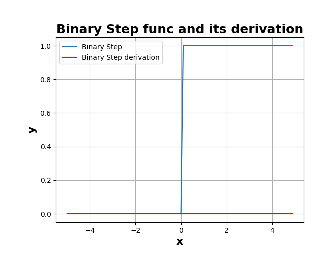
\includegraphics[width=0.6\textwidth]{content/chapter_basics/plots/binary_step_func_plot.eps}
	\centering
	\caption{Graph der Funktion \textit{Binary Step} und deren Ableitung}
	\label{img:binary_step_func_graph}
\end{figure}

Ein Problem, welches ebenfalls in \cite[311-312]{sharma-2020} beschrieben wird, ist das der Gradient für $x$ Null ist. Dieser Umstand kann dazu führen, dass die Backpropagation nicht ausgeführt werden kann.\vspace{0.2cm}

%%----------------------------------------------------------------------------
%   Sigmoid
%
\textbf{Sigmoidfunktion}\vspace{0.2cm}

Die Sigmoidfunktion ist eine der bekanntesten Aktivierungsfunktionen und eine Sonderform der logarithmischen Funktion. Ein Eingangswert $x$ liefert einen garantierten Ausgabewert zwischen $null$ und $eins$. Sie ist monoton steigend und überall differenzierbar. Der Einsatz der Sigmoidfunktion als Aktivierungsfunktion in einer Hidden-Schicht ermöglicht dem neuronalen Netz eine nicht lineare Trennbarkeit im 2-dimensionalen zu lernen. Ebenfalls ermöglichen ihre Eigenschaften, bei kleinen Netzwerktiefen den Backpropagation-Algorithmus einfach anzuwenden und ermöglicht das Lernen des Netzwerks. Bei großen Netzwerken mit vielen Schichten kann es aber zum \glqq Problem der verschwindenden Gradienten\grqq \ führen auch bekannt als \textit{Vanishing-Gradient-Problems}. Es ist bekannt, dass die Ableitung der Sigmoidfunktion einen Maximalwert von $0,25$ annehmen kann. Bei mehreren Schichten wird das Produkt der Ableitung immer kleine bis dieser sich $null$ annähert.\vspace{0.2cm}

Die Formel \ref{eq:sigmoid_function} zeigt die Sigmoidfunktion, die Formel \ref{eq:derivative_sigmoid_function} die erste Ableitung der Sigmoidfunktion.

%\begin{equation}\label{eq:sigmoid_function}
%	\sigma (x) = sig(x) = \frac{1}{1 + e^{-x}}
%\end{equation}
\xequation{Sigmoid Funktion}{\label{eq:sigmoid_function}
	\sigma (x) = sig(x) = \frac{1}{1 + e^{-x}}
}

%\begin{equation}\label{eq:derivative_sigmoid_function}
%	\sigma' (x) = sig(x) * (1 - sig(x))
%\end{equation}
\xequation{Ableitung: Sigmoid Funktion}{\label{eq:derivative_sigmoid_function}
	\sigma' (x) = sig(x) * (1 - sig(x))}

Der Graph der Sigmoidfunktion und ihre Ableitung ist in Abbildung \ref{img:sig_func_graph} dargestellt. Hierbei ist zu erkennen, dass die Ableitung eine Symmetrie im Ursprung zeigt. Im Ursprung die maximale Steigung zu finden ist und für kleine und große $x$-Werte gegen $null$ konvergiert.

\begin{figure}[!ht]
	\includegraphics[width=0.6\textwidth]{content/chapter_basics/plots/sigmoid_func_plot.eps}
	\centering
	\caption{Graph Sigmoidfunktion und deren Ableitung}
	\label{img:sig_func_graph}
\end{figure}

Diese Funktion hat zwei Nachteile. Zum einen bei kleinen und großen Werten, konvergiert der Gradient gegen null. Somit wird die Verlustfunktion sehr klein und die Aktualisierung der Gewichte während des Lernens wird verhindert.\vspace{0.2cm}

%%----------------------------------------------------------------------------
%   tanh
%
\textbf{Tangens Hyperbolicus}\vspace{0.2cm}

Ebenso wie die Sigmoidfunktion ist auch die Tangens Hyperbolicus eine monoton stetig steigende Funktion, die symmetrisch zum Ursprung ist. Der Ausgabewert liegt garantiert hier zwischen $-1$ und $1$, was dazu beiträgt, dass die Ausgabe der Schicht um eins zentriert bleibt, welches ein Vorteil bei Normalisierung der Ausgabewerte ist. Auch hier haben wir, in tiefen Netzen das \glqq Problem des verschwindenden Gradienten\grqq \ wie bei der Sigmoidfunktion. In flachen Netzen erleichtern die Eigenschaften den Optimierungsprozess.\vspace{0.2cm}

%\begin{equation}\label{eq:tanh_function}
%	\sigma (x) = tanh(x) = \frac{e^{x} - e^{-x}}{e^{x} - e^{-x}}
%\end{equation}
\xequation{Tangenshyperbolicus Funktion}{\label{eq:tanh_function}
	\sigma (x) = tanh(x) = \frac{e^{x} - e^{-x}}{e^{x} - e^{-x}}
}

%\begin{equation}\label{eq:derivative_tanh_function}
%	\sigma' (x) = tanh^2(x)
%\end{equation}
\xequation{Ableitung: Tangenshyperbolicus Funktion}{\label{eq:derivative_tanh_function}
	\sigma' (x) = tanh^2(x)
}

Die Abbildung \ref{eq:tanh_function} zeigt den Graphen der Tangens Hyperbolicus Funktion und deren Ableitung. Deutlich zu erkennen ist die Symmetrie zum Ursprung bei der Ableitung, hier rot dargestellt.

\begin{figure}[!ht]
	\includegraphics[width=0.6\textwidth]{content/chapter_basics/plots/tanh_func_plot.eps}
	\centering
	\caption{Graph Tangens Hyperbolicus und deren Ableitung}
	\label{img:tanh_func_graph}
\end{figure}

Die Verwendung der Tangens Hyperbolicus als Aktivierungsfunktion kann bei sehr großen Netzen zu sehr rechenintensiven Prozessen führen, da wie in der Formel \ref{eq:tanh_function} zu erkennen ist, die Exponentialfunktion oft verwendet wird.\vspace{0.2cm}

%%----------------------------------------------------------------------------
%   ReLU
%
\textbf{ReLU}\vspace{0.2cm}

% https://machinelearningmastery.com/activation-functions-in-pytorch/

Die Rectified Linear Unit (ReLU) ist eine weitere weit verbreitete Aktivierungsfunktion. Bei dieser Funktion handelt es sich um eine gesättigte Funktion, da bei unendlich großen $x$ die Ausgabe gegen unendlich geht, siehe Formel \ref{eq:non_saturating_relu}, hingegen bei Eingaben $x < 0$ die Ausgabe immer $null$ liefert, vgl. mit Formel \ref{eq:relu_function}. Diese Funktion gehört ebenfalls zu den nicht linearen Aktivierungsfunktionen. Laut \cite{yuen_universal_2021} ist die Funktion linear, allerdings nur bei positiven Eingangsignalen.\vspace{0.2cm}

%\begin{equation}\label{eq:non_saturating_relu}
%	\lim_{z -> \infty} \sigma(x) = + \infty
%\end{equation}
\xequation{Nicht sättigende ReLU Funktion}{\label{eq:non_saturating_relu}
	\lim_{z -> \infty} \sigma(x) = + \infty
}

Wie in \cite{yuen_universal_2021} beschrieben wird diese Funktion bei Quantifizierungs-, Klassifizierungs- und Verstärkungslernproblemen verwendet. Bei Quantisierungsproblemen wird versucht die Ausgaben auf wenige diskrete Stufen zu reduzieren. Da viele Eingaben durch ReLU Funktion eine Ausgabe von $null$ erzeugen (auch bekannt als: Prinzip der geringen Wirkung [engl. Sparsity Effect]), werden auf natürlichem Wege eine Menge an Signalen eliminiert, was ein Vorteil für die Quantisierung darstellt. Durch ihr nicht lineares Verhalten ist diese Funktion auch für Klassifizierungsprobleme effizient. Häufig wird beobachtet das, bei Verstärkungsproblemen ein Rückgang des Gradienten erfolgt. Da die ReLU das \textit{Problem des verschwindenden Gradienten} mildert, schafft sie dadurch eine stabile Lernumgebung. Zudem werden unnötige Aktionen durch das \textit{Prinzip der geringen Wirkung} vermieden.

%\begin{equation}\label{eq:relu_function}
%	\sigma (x) = \left\{
%	\begin{array}{cl}
%		x & : \ x > 0 \\
%		0 & : \ x \leq 0
%	\end{array}
%	\right.
%\end{equation}
\xequation{ReLU Funktion}{\label{eq:relu_function}
	\sigma (x) = \left\{
	\begin{array}{cl}
		x & : \ x > 0 \\
		0 & : \ x \leq 0
	\end{array}
	\right.
}

%\begin{equation}\label{eq:derivative_relu_function}
%	\sigma' (x) = \left\{
%	\begin{array}{cl}
%		1 & : \ x > 0 \\
%		0 & : \ x \leq 0
%	\end{array}
%	\right.
%\end{equation}
\xequation{Ableitung: ReLU Funktion}{\label{eq:derivative_relu_function}
	\sigma' (x) = \left\{
	\begin{array}{cl}
		1 & : \ x > 0 \\
		0 & : \ x \leq 0
	\end{array}
	\right.
}

Die Abbildung \ref{eq:relu_function} zeigt die Graphen der ReLU Funktion und dessen Ableitung. Bei Eingaben kleiner als $null$ liefert die Funktion immer $null$ als Ausgabe.

\begin{figure}[!ht]
	\includegraphics[width=0.6\textwidth]{content/chapter_basics/plots/relu_func_plot.eps}
	\centering
	\caption{Graph ReLU und deren Ableitung}
	\label{img:relu_func_graph}
\end{figure}

Die folgenden Eigenschaften sind \cite{cs231n_2024} entnommen. Es wurde festgestellt, dass die ReLU-Funktion die Konvergenz des Gradientenabstiegs, aufgrund seiner linearen, nicht gesättigten Form stark beschleunigt. Da die Funktion keine Exponentialfunktion ist, sind die Kosten bei der Berechnung relativ gering. Ein Nachteil dieser Funktion ist bei sehr großen Gradienten zu sehen. Hierbei kann es passieren, das die Gewichte so aktualisiert werden, dass das Neuron nie wieder aktiviert wird und immer $null$ als Ausgabe hat. In diesem Fall können ganze Teile des Netzwerk \glqq Tot\grqq \ bleiben. 
\vspace{0.2cm}

Wie \cite{yuen_universal_2021} entnommen kann es vorkommen, dass das Gradientenabstiegsoptimierung abstürzt. Der Grund ist, dass diese Funktion eine Diskontinuität bei $x=0$ besitzt, was zu einem undefinierten Gradienten führt.\vspace{0.2cm} 

%%----------------------------------------------------------------------------
%   Leaky ReLU
%
\textbf{Leaky ReLU}\vspace{0.2cm}

Bei der Leaky ReLU handelt es sich um eine Variante der ReLU Funktion. Wie auch bei der ReLU ist die Leaky ReLU eine nicht lineare stetige Funktion, auch im Bereich von $x = 0$, was bei dem Optimierungsprozess, auch bei tiefen Netzen hilfreich sein kann. In Sachen Effizienz ist die Leaky ReLU mit der einfachen ReLU vergleichbar.\vspace{0.2cm}

An dieser Stelle sei noch die parametrische ReLU, PreLU erwähnt. Bei der PReLU ist der Parameter $\alpha$ nicht fest hinterlegt, sondern kann beim Training, wie ein Bias aktualisiert werden. Die Tabelle \ref{tab:relu_types_differents} zeigt eine Zusammenfassung der Unterschiede und ist \cite{bhargav-2023} entnommen.

\begin{center}
	\begin{table}[!ht]
		\begin{tabular}{>{\small}l>{\small}l>{\small}l>{\small}l}
			& \textbf{ReLU} & \textbf{LReLU} & \textbf{PReLU} \\
			\hline
			Vorteil & Löst Gradientenprobleme & Löst Gradienten- & Löst Gradienten- \\
			&& probleme & probleme \\
			Nachteil & Sterbendes Relu-Problem & Inkonsistente Ausgabe & Feinabstimmung $\alpha$ \\
			&& für negative Eingabe & \\
			Hyperparamete & nein & nein & ja \\
			Geschwindigkeit schnell& schneller & am schnellsten & \\
			Genauigkeit & hoch& höher & am höchsten \\
			Konvergenz & langsam & schnell & am schnellsten \\
		\end{tabular}
		\caption{Wichtige Unterschiede von ReLU Aktivierungsfunktionen}
		\label{tab:relu_types_differents}
	\end{table}
\end{center}

Da diese Funktion auch bei negativen $x$-Werten einen Gradienten ungleich $null$ besitzt, wird das \glqq Problem der verschwindenden Gradienten\grqq \ umgangen und somit wird auch das Problem der \glqq toten Neuronen\grqq \ verringert. Die Formel \ref{eq:derivative_leaky_relu_function} zeigt diese Eigenschaft. Da Alpha einen sehr geringen Wert hat, kann es dennoch passieren, dass bei sehr tiefen Netzen das Lernen sehr langsam verläuft. Ein weiterer Nachteil der Funktion sind die positiven Werte welche keinerlei Begrenzung besitzen, dieses Problem wird in Formel \ref{eq:leaky_relu_function} deutlich. Bei extrem großen Werten kann es im Netzwerk zu nummerischen Problemen führen.

%\begin{equation}\label{eq:leaky_relu_function}
%	\sigma (x) = \left\{
%	\begin{array}{cl}
%		x & : \ x > 0 \\
%		\alpha x & : \ x \leq 0
%	\end{array}
%	\right.
%\end{equation}
\xequation{Leaky ReLU Funktion}{\label{eq:leaky_relu_function}
	\sigma (x) = \left\{
	\begin{array}{cl}
		x & : \ x > 0 \\
		\alpha x & : \ x \leq 0
	\end{array}
	\right.
}

%\begin{equation}\label{eq:derivative_leaky_relu_function}
%	\sigma' (x) = \left\{
%	\begin{array}{cl}
%		1 & : \ x > 0 \\
%		\alpha & : \ x \leq 0
%	\end{array}
%	\right.
%\end{equation}
\xequation{Ableitung: Leaky ReLU Funktion}{\label{eq:derivative_leaky_relu_function}
	\sigma' (x) = \left\{
	\begin{array}{cl}
		1 & : \ x > 0 \\
		\alpha & : \ x \leq 0
	\end{array}
	\right.
}

Die Abbildung \ref{img:leaky_relu_func_graph} zeigt den Graphen der Leaky ReLU Funktion mit einem $\alpha$-Wert von 0,2. Ebenso ist die Ableitung dieser Funktion zu sehen, als roter Graph dargestellt.

\begin{figure}[!ht]
	\includegraphics[width=0.6\textwidth]{content/chapter_basics/plots/leaky_relu_func_plot.eps}
	\centering
	\caption{Graph Leaky ReLU und deren Ableitung}
	\label{img:leaky_relu_func_graph}
\end{figure}

Der Einsatz der Leaky ReLU gegenüber der Standard ReLU, kann bei sehr tiefen neuronalen Netzen erfolgen. wenn es um sehr komplexe Klassifizierungsprobleme geht oder wenn die Standard-ReLU nicht funktioniert, beispielsweise wenn festgestellt werden kann, dass sehr viele inaktive Neuronen während des Trainings entstehen. Ein weiteres Beispiel bei der die Leaky ReLU verwendet werden sollte wird in \cite{rallabandi-2023} genannt. Es wird empfohlen die Leaky ReLU zu verwenden, wenn die Daten ein großes Rauschen oder viele Ausreißer aufweisen.\vspace{0.2cm}

%%----------------------------------------------------------------------------
%   Gaussian
%
\textbf{Gaußfunktion}\vspace{0.2cm}

Abgeleitet wird diese Aktivierungsfunktion von der Gaußschen Normalverteilung ab und symmetrisch um den Ursprung. Somit werden für kleine positive und negative Eingabewerte, hohe Ausgabewerte und für hohe positive und negative Eingangswerte niedrige Ausgangswerte erzeugt. Daraus folgt die stärkste Aktivierung der Neuronen erfolgt bei Werten nahe dem Ursprung. Die Ausgaben liegen zwischen $null$ und $eins$. Sie ist stetig und unendlich oft differenzierbar. Diese Eigenschaft ist ein Vorteil für den Gradientenabsteig. Die Gaußfunktion ist wie Sigmoid oder Tangens Hyperbolicus sehr rechenintensiv, aufgrund Verwendung der Exponentialfunktion.\vspace{0.2cm}

Die Gaußfunktion wird in neuronalen Netzen verwendet, die zur Mustererkennung und Klassifikation dienen. Hierbei handelt es sich um eine radiale Aktivierungsfunktion, bekannt als \textit{Radial Basis Function} (\acrshort{RBF}).

%\begin{equation}\label{eq:gaussian_function}
%	\sigma (x) = e^{-x^{2}}
%\end{equation}
\xequation{Gaussfunktion}{\label{eq:gaussian_function}
	\sigma (x) = e^{-x^{2}}
}

%\begin{equation}\label{eq:derivative_gaussian_function}
%	\sigma' (x) = -2x e^{-x^{2}}
%\end{equation}
\xequation{Ableitung Gaussfunktion}{\label{eq:derivative_gaussian_function}
	\sigma' (x) = -2x e^{-x^{2}}
}

In der Abbildung \ref{img:gaussian_func_graph} zeigt den Graphen der Gaußfunktion und dessen Ableitung. Hier ist zu erkennen, dass die Ableitung eine Antisymmetrie um den Ursprung aufweist, was mit $f'(-x) = -f'(x)$ ausgedrückt werden kann. Ebenfalls strebt die Ableitung für sehr kleine und sehr große $x$-Werte schnell gegen $null$, was das \glqq Problem der verschwindenden Gradienten \grqq \ begünstigt.

\begin{figure}[!ht]
	\includegraphics[width=0.6\textwidth]{content/chapter_basics/plots/gaussian_func_plot.eps}
	\centering
	\caption{Graph Gaußfunktion und deren Ableitung}
	\label{img:gaussian_func_graph}
\end{figure}

Ein Nachteil der Gaußfunktion kann entsteht bei sehr tiefen neuronalen Netzen. Hier kann die schnell wegen ihrer gegen $null$ strebende Natur, zur eine Abnahme oder zum Erliegen der Aktivierungen von nachfolgenden Neuronen kommen und das Training erschweren. Die Gaußfunktion finden in den Standardnetzwerken eher wenig Anwendung. Ihre Stärken kommen erst in speziellen Netzen wie das RBF-Netz zur Geltung, wo ihre lokalen Aktivierungseigenschaften optimal genutzt werden können.\vspace{0.2cm}

%%----------------------------------------------------------------------------
%   Softmax
%
\textbf{Softmax}\vspace{0.2cm}

% https://arxiv.org/pdf/1302.4389v4, https://arxiv.org/abs/1302.4389v4
% https://arxiv.org/pdf/2208.04468

Die Softmax Aktivierungsfunktionen wird häufig in der Ausgabeschicht eines neuronalen Netzes eingesetzt. Als Eingang dient nicht ein einzelnes Signal, wie bei den zuvor vorgestellten Funktionen, viel mehr werden alle Ausgaben der vorherigen Schicht verwendet, um Prognosen zu erstellen.

%\begin{equation}\label{eq:softmax_function}
%	\sigma (x)_{j} = softmax(x_{j}) = \frac{e^{z_{j}}}{\sum_{k=1}^{K} e^{z_{k}}} \text{ für } j = 1, ..., K.
%\end{equation}
\xequation{Softmax Funktion}{\label{eq:softmax_function}
	\sigma (x)_{j} = softmax(x_{j}) = \frac{e^{z_{j}}}{\sum_{k=1}^{K} e^{z_{k}}} \text{ für } j = 1, ..., K.
}

Als Ausgabe wird ein Vektor erstellt der die prozentuale Verteilung der Eingangswerte darstellt. Zusammen ergeben die Ausgaben 1, also 100\%, welches Formel \ref{eq:softmax_result} zeigt.

%\begin{equation}\label{eq:softmax_result}
%	\sum_{i=1}^{k} softmax(z_{j}) = 1
%\end{equation}
\xequation{Ableitung: Softmax Funktion}{\label{eq:softmax_result}
	\sum_{i=1}^{k} softmax(z_{j}) = 1
}

Die Softmax wird hauptsächlich angewandt, um Klassifizierungsprobleme die aus mehreren Klassen bestehen zu lösen. Für die eine Wahrscheinlichkeitsverteilung errechnet wird. Durch ihre Differenzierbarkeit kann der Backpropagation-Algorithmus angewandt werden, um die Gewichte zu optimieren.\vspace{0.2cm}

Nachteilig auf die Softmax-Funktion wirken sich Ausreißer aus. Eine deutlich größeres Eingangssignal kann dominieren, auch wenn es nicht korrekt ist. Was zu einer Fehlinterpretation der Vorhersage kommen.\vspace{0.2cm}

%%----------------------------------------------------------------------------
%   Maxout
%
\textbf{Maxout}\vspace{0.2cm}

Die Maxout ist ein leistungsstarkes Modell welches in \cite{goodfellow_maxout_2013} vorgestellte wurde und dient zur Ergänzung der Dropout-Technik. Die Funktion verwendet für die Berechnung genau wie die Softmax, die Ausgaben von Neuronen der vorherigen Schicht. Jedes Maxout-Neuron hat mehrere Transformationsvektoren und einen Bias-Vektor. Jede Transformation erhält seinen eigenen Bias-Wert. Aus den Berechnungen sucht der Algorithmus das Maximum aus den Ergebnissen heraus und liefert dieses als Output. Die Formel \ref{eq:maxout_function} zeigt den Maxout.

%\begin{equation}\label{eq:maxout_function}
%	\sigma (x)_{j} = max(\omega^T_1 x + b_1, \omega^T_2 x + b_2, ..., \omega^T_j x + b_j)
%\end{equation}
\xequation{Maxout-Funktion}{\label{eq:maxout_function}
	\sigma (x)_{j} = max(\omega^T_1 x + b_1, \omega^T_2 x + b_2, ..., \omega^T_j x + b_j)
}

Bei der Dropout Technik handelt es sich um ein Verfahren welches beim Training neuronaler Netze angewandt wird. Es soll das \gls{overfitting} verhindern. Durch dieses Verfahren sollen Modelle robuster und die Abhängigkeit von einzelnen Neuronen soll vermieden werden. Im Trainer kommt es zum Deaktivieren einzelner zufällig ausgewählter Neuronen. Das Verfahren ist besonders bei tiefen Netzen mit vielen Parametern nützlich.


%\subsubsection{Schichten im neuronalen Netz}
%In den meisten Netzen gibt es eine Eingangsschicht (Input layer), eine bis mehrere versteckte Schichten (Hidden layer) und eine Ausgangsschicht (Output layer). Die Schichten bestehen aus einer Reihe von künstlichen Neuronen. Zwischen den Schichten sind Verbindungen zu deren Neuronen. Diese können vorwärts, also vom Eingang zum Ausgang oder rückwärts gerichtet sein.

\subsubsection{Arten der neuronalen Netzen}
Neuronale Netze bestehen meist aus mehreren Schichten. Die Schichten wiederum enthalten eine definierte Menge an Neuronen und können in drei Arten eingeteilt werden. Die Eingabeschicht (Input layer) nimmt die Daten $\overrightarrow{x}=(x_{1}, ..., x_{n})^T$ für das Netzwerk entgegen. In einigen Netzen werden diese Daten in dieser Schicht normalisiert. Nach der Eingabeschicht folgen ein oder mehrere versteckte Schichten (Hidden layer), welche die Daten verarbeiten. Zum Schluss kommt die Ausgabeschicht (Output layer) die die Ergebnisse $\overrightarrow{y}=(y_{1}, ..., y_{n})^T$ des Netzwerks bereitstellt.

% https://datasolut.com/neuronale-netzwerke-einfuehrung/

\begin{figure}[!ht]
	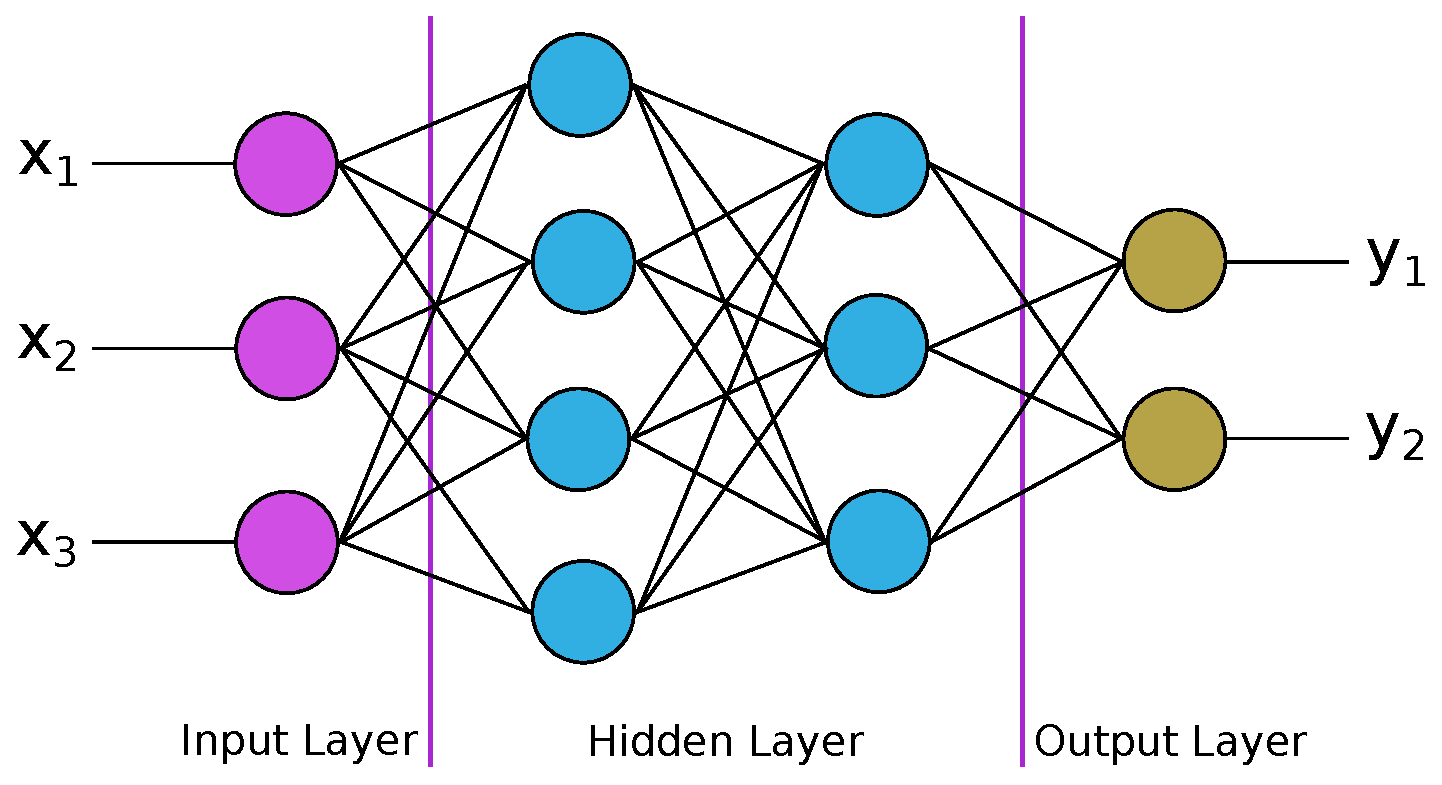
\includegraphics[width=0.6\textwidth]{content/chapter_basics/images/neuronal_network.eps}
	\centering
	\caption{Aufbau eines neuronalen Netzwerkes}
	\label{img:neural_network}
\end{figure}

Alle Verbindungen oder nur ausgesuchte.\vspace{0.2cm}

Im Folgenden werden einige neuronale Netze vorgestellt.\vspace{0.2cm}

\textbf{Einschichtige Netze (Perzeptrons)}\vspace{0.2cm}

\textbf{Feedforward Neural Netzwerke (FNN)}\vspace{0.2cm}
%https://artemoppermann.com/de/neuronale-netze-und-ihre-anwendungen/
Ein FNN besteht aus einer Eingabeschicht, mindestens einer versteckten Schicht und einer Ausgabeschicht. Ein FNN ist in der Struktur und Aufbau vergleichbar mit Abbildung \ref{img:neural_network_fnn}. Ein FNN hat in der Eingabeschicht genau so viele Neuronen wie Eingangswerte der Daten. Alle anderen Schichten können beliebig viele Neuronen enthalten. Da eine Schicht immer nur mit der nachfolgenden verbunden ist, fließen die Daten in diesem Netzwerk nur in eine Richtung. Somit können bereits verarbeitete Daten nicht noch einmal für eine weitere Verarbeitung herangezogen werden.

\begin{figure}[!ht]
	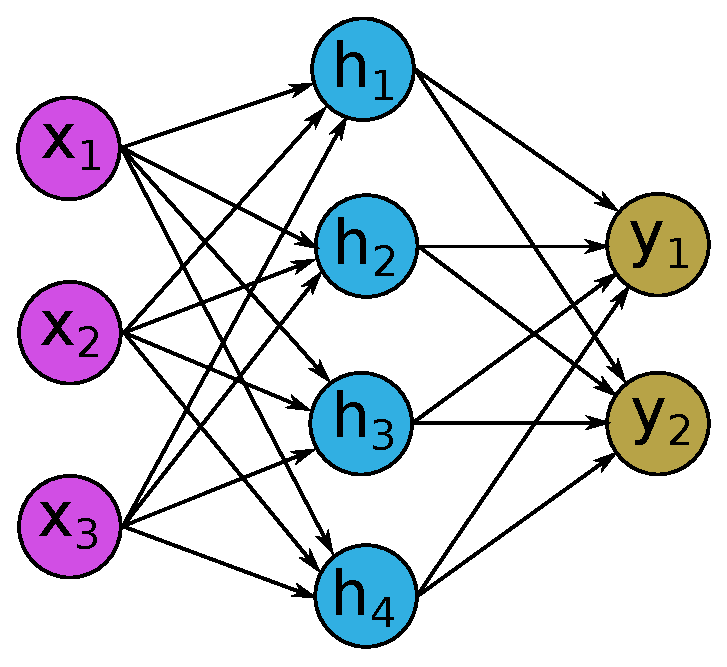
\includegraphics[width=0.4\textwidth]{content/chapter_basics/images/neuronal_network_fnn.eps}
	\centering
	\caption{Aufbau eines FNN}
	\label{img:neural_network_fnn}
\end{figure}

FNNs in vielen Bereichen eingesetzt, so beispielsweise bei der Bild- und Spracherkennung, aber auch bei Vorhersagen und Entscheidungsfindung.\vspace{0.2cm}

\textbf{Rekurrente neuronale Netze (RNNs)}\vspace{0.2cm}

\begin{figure}[!ht]
	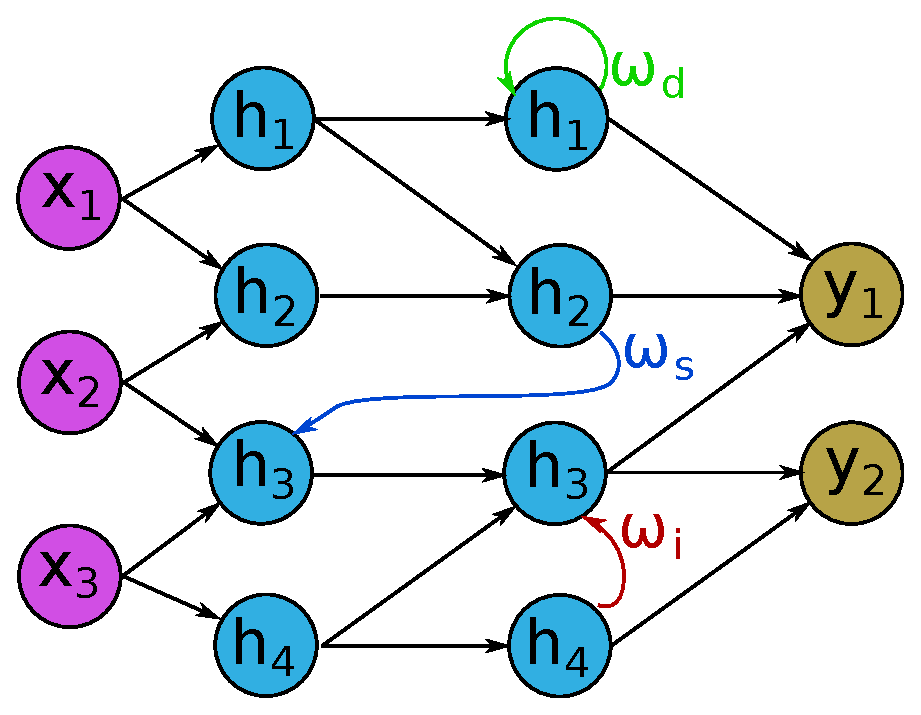
\includegraphics[width=0.4\textwidth]{content/chapter_basics/images/neuronal_network_rnn.eps}
	\centering
	\caption{Aufbau eines RNN mit möglichem rückwärts gerichteten Verbindungen}
	\label{img:neural_network_rnn}
\end{figure}

%\textbf{Convolutional Neural Networks (CNNs)}\vspace{0.2cm}

%\textbf{Long Short-Term Memory Networks (LSTM)}\vspace{0.2cm}

%\textbf{Recurrent Convolutional Neural Networks (RCNNs)}\vspace{0.2cm}


\subsubsection{Lernprozess im neuronalen Netz / Training}
% hier entnommen: https://www.datacamp.com/tutorial/mastering-backpropagation?dc_referrer=https%3A%2F%2Fwww.bing.com%2F#rdl

Ein wichtiger Bestandteil im überwachten Training für neuronale Netzwerke ist die Backpropagation. Hierbei wird die Fehlerrate, welcher durch die Vorwärtspropagation entsteht, rückwärts durch das Netz propagiert und die Gewichte werden aktualisiert. Für das Training sind Trainingsdaten notwendig, bei denen die Ergebnisse bekannt sind, welches zum Errechnen der Fehlerrate erforderlich sind. Dieser Verlust wird dann rückwärts durch das Netz propagiert. Das am häufigste angewandte Verfahren ist das \gls{gated_recurrent_unit}.\vspace{0.2cm}

Insgesamt kann der Backpropagation-Algorithmus in vier Teilschritte unterteilt werden.\vspace{0.2cm}

\textit{Vorwärtspropagation}: Zuerst werden die Trainingsdaten an das Netzwerk übergeben und die Berechnung des Ergebnisses kann erfolgen. Die Berechnung erfolgt anhand der vorgegebenen Gewichte, diese werden mit den jeweiligen Eingängen multipliziert und mit dem Bias-Wert addiert. Zum Schluss steht ein Ergebnis fest, welches am Anfang mit hoher Wahrscheinlichkeit vom erwarteten Ergebnis abweicht.\vspace{0.2cm}

\textit{Fehlerberechnung}: Das tatsächliche Ergebnis wird mit dem erwarteten Ergebnis verglichen und die Differenz gebildet. Hieraus ergibt sich der Fehler des Netzwerkes.\vspace{0.2cm}

\textit{Rückwätspropagation}: Der errechnete Fehlerwert wird zur Berechnung des Gradienten verwendet. Das Ergebnis wird dann von der Ausgangsschicht durch das Netz rückwärts propagiert und Bezug auf jedes einzelne Gewicht genommen, um die Änderung des jeweiligen Gewichtes zu errechnen.\vspace{0.2cm}

\textit{Gewichte aktualisieren}: Um die Größe der Änderung zu bestimmen wird eine Lernrate benötigt, welche die maximale Änderung der Gewichte vorgibt. Nun werden die Gewichte in entgegengesetzter Richtung des Gradienten angepasst, wodurch das Verfahren den Namen \glqq Gradienabstieg\grqq \ erhielt.\vspace{0.2cm}

Dieses Verfahren wiederholt, bis die \textit{Anzahl der Epochen} erreicht ist. Die \glqq Anzahl der Epochen \grqq \ ist ein weiterer Wert für die Backpropagation erforderlich ist. Wird Wahl der Epochen zu gering gewählt ist das Model nicht ausreichend trainiert, eine zu hohe Anzahl zieht das Training in Läge ohne maßgebliche Erfolge zu verzeichnen.\vspace{0.2cm}

Die Backpropagation bring einige Vorteile. Sie ist einfach zu implementieren, da für fast jede Sprache eine entsprechende Library existiert. Des Weiten ist der Algorithmus flexibel und lässt sich leicht an verschiedenen Netzwerke und Architekturen anpassen und deckt somit ein weites Spektrum im Bereich KI ab. Ein weiterer Vorteil ist, es werden keine zusätzlichen Parameter benötigt, es genügen die Trainingsdaten.\vspace{0.2cm}

Er bringt aber einige Einschränkungen mit sich. So wird ein Modell schlecht trainiert, wenn die Datenqualität ungenügend ist. Dazu zählen Rauschen, unvollständig und verzerrte Daten. Bei sehr tiefen Netzen, kann die Trainingsdauer sehr viel Zeit in Anspruch nehmen, was sich in einigen Fällen als unpraktisch erweisen kann. Durch den Matrix-basierten Ansatz steigt der Rechenbedarf mit steigender Netztiefe, was möglicherweise an die Ressourcengrenze der Hardware stößt.

\subsection{Deep Learning}
Der Bereich Deep Learning \acrshort{DL} ist ein Bestandteil der Bereiche ML und KI. Hierbei werden tiefe neuronale Netze verwende, mit vielen Hidden Layer, um eine umfangreiche innere Struktur zu bilden. Dadurch können große Mengen an Daten effizient verarbeitet und Datenmuster erkannt werden.\vspace{0.2cm}

Mithilfe von DL werden Problem im Bereich Klassifizierung, Regression und Vorhersagen gelöst.

% aus: https://engineering.purdue.edu/~ersoy/sa10503_su24/days/day6/matlab_Deep_Learning_ebook.pdf
\epigraph[
author={MathWorks},
source={Introducing Deep Learning with MATLAB}
]{
	Deep learning is a type of machine learning in which a model learns to perform classification tasks directly from images, text, or sound. Deep learning is usually implemented using a neural network architecture. The term “deep” refers to the number of layers in the network—the more layers, the deeper the network. Traditional neural networks contain only 2 or 3 layers, while deep networks can have hundreds.
}

% aus: https://arxiv.org/pdf/2104.05314
% main: https://arxiv.org/abs/2104.05314
In ?? wird \textit{Depp Learning}, aufbauend auf einer \textit{Machine Learning} Aussage beschrieben als,

\epigraph[
author={Schmidhuber},
source={Deep Learning}
]{
	Machine learning describes the capacity of systems to learn from problem-specific training data to automate the process of analytical model building and solve associated tasks. Deep learning is a machine learning concept based on artificial neural networks. For many applications, deep learning models outperform shallow machine learning models and traditional data analysis approaches.
}

\subsection{Natural Language Processing}
Das Feld der Natural Language Processing, kurz \acrshort{NLP} ist ein Teilgebiet Künstlichen Intelligenz und ein Teilgebiet in Deep Learning. NLP soll es digitalen Geräten ermöglichen kodierte Texte und Sprachen zu erkennen, zu verstehen und zu generieren. Dabei muss NLP die Bedeutung (Semantik) erkennen. Sie muss Grammatik kennen und Beziehungen zwischen Teilen der Sprache herstellen. Sie Wortarten wie Verben, Adjektive und Nomen spezifizieren. Sie muss verschiedene Formen der Sprache Prosa beherrschen wie Prosa oder wissenschaftliches Schreiben.\vspace{0.2cm}

Erste große Erfolge haben NLP mit neuronalen Netzen wie den \textit{Feedforward Neural Networks} und \textit{Convolutional Neural Networks}, wie in \cite{goldberg-2016} zeigt. Mit der Einführung von GPT und BERT, wurde bei dem NLP die neuen Transformer Modellen verwendet.

\section{Large Language Model}
Die Teilgebiete Deep Learning und Natural Language Processing haben es den großen Sprachmodellen \acrshort{LLM} ermöglicht kommunikationsfähig zu werden. Sie verstehen Anfragen und können Antworten generieren. Die LLMs sind in der Lage Bilder und andere Medien wie Video oder Audio zu generieren.\vspace{0.2cm}

Diese Modelle wurden mit sehr großen Datenmengen trainiert und sind daher in der Lage natürliche Sprache zu verstehen.

\subsection{Grundlagen}
%Die großen Sprachmodelle oder Large Language Models sind darauf ausgelegt menschliche Sprache zu verstehen. Durch Textanalyse und Verarbeitung der Textbausteine durch \textit{Tokenisierung} und Vorhersage kommender Textbausteine.\vspace{0.2cm}

Die großen Sprachmodelle können menschliche Sprache arbeiten. Sie sind speziell für die Lösung  sprachbezogene Probleme geeignet, wie Textgenerierung, Klassifizierung und Übersetzung. Sie nehmen Anfragen sog. \textit{Prompts} entgegen und errechnen daraus die wahrscheinlichste Antwort. Des Weiteren können Prompts als Anweisung (instruction-tuning) oder in Dialogform (chat fine-tuning) gestellt werden. Die heutigen Sprachmodelle sind Modelle, welche die Transformer Technik verwenden.

Die grundlegende Funktionsweise der Large Language Models kann in vier Hauptkomponenten unterteilt werden,

\begin{enumerate}
	\item Tokenisierung: zerlegen der Texte in einzelne Token
	\item Embedding: Vergleiche mit anderen Vektoren und Einordnung in einer Gesamtstruktur
	\item Vorhersage: Wahrscheinlichkeit des nächsten Tokens berechnen
	\item Dekodierung: Auswahl der Ausgabestrategie
\end{enumerate}

Die folgenden Unterpunkte erläutern die Hauptkomponenten näher.

\subsubsection{Tokenisierung}
Der erste Schritt besteht darin die eingegebenen Texte zu zerlegen. Die Zerlegung kann unterschiedlich gestaltet sein. Von einzelnen Zeichen, über Teilworte bis hin zu ganzen Worten. Welche Zerlegung gewählt wird, hängt maßgeblich von zwei verschiedenen Parametern ab. Zum Einem welcher Informationsgehalt ist in einem Token enthalten. Beispielsweise haben einzelne Zeichen nicht den gleichen Informationsgehalt wie ganze Worte. Der andere Aspekt ist die Anzahl der Tokens. Für ASCII bräuchte man  Token, für die Worte aus der deutschen Sprache benötigt man, laut \cite{duden_unknown-author} etwa 300'000 bis 600'000 Token.\vspace{0.2cm}

Der im Listing \ref{lst:javascript_metho_api_call} zu sehen Methodenausschnitt einer JavaScript-Methode, wird mithilfe der Tokenisierung wie in Abbildung \ref{img:tokenize_javascript_method} gezeigt, zerlegt.

\begin{center}
	\begin{lstlisting}[
		language=JavaScript,
		caption={JavaScript Methode für einen API Aufruf},
		label={lst:javascript_metho_api_call}]
		async function fetchUserData(apiUrl) {
			try {
				const response = await fetch(apiUrl);
				if (!response.ok) {
					throw new Error(
					'HTTP error! Status: ${response.status}'
					);
				}
				console.log('${response.status}')
				const data = await response.json();
				return data;
			} catch (error) {
				console.error("Fehler beim Abrufen:", error);
				return null;
			}
		}
	\end{lstlisting}
\end{center}

In der Abbildung \ref{img:tokenize_javascript_method} ist die Tokenisierung mittel Wortteilen zu erkennen. Diese Tokenisierung wurde mit \href{https://tiktokenizer.vercel.app/}{https://tiktokenizer.vercel.app/} erstellt und das Model \textit{codellama/CodeLlama-70b-hf} verwendet.

\begin{center}
	\begin{figure}[!ht]
		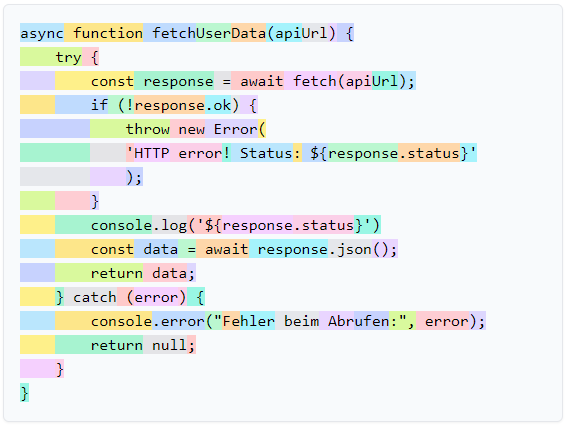
\includegraphics[width=0.7\textwidth]{content/chapter_basics/images/tokenize.png}
		\centering
		\caption{Tokenisierung einer JavaScript-Methode}
		\label{img:tokenize_javascript_method}
	\end{figure}
\end{center}

Die Tokenisierung von Quellcode stellt besondere Anforderungen. Hier muss die Sprache erkannt werden, um die Verwendung verschiedener Keywords zu realisieren. Ebenfalls müssen unterschiedliche Operatoren und Strukturen angewandt werden, z.B. \code{===} in JavaScript und \code{::} in PHP. Bei natürlicher Sprache leite sich die Bedeutungen der Worte durch den Kontext ab, während er bei Programmcode konsistent verarbeite werden muss. Die Semantik muss erhalten bleiben, sodass Variablennamen ihre spezifische Bedeutung behalten und die Rolle Sonderzeichen muss beachtet werden. Beispielsweise für Klammern aller Art und auch für das Semikolon. Mathematische Symbole spielen ebenso eine wichtige Rolle, wie mehrdeutige Symbole wie \code{*} (bezeichnet in C/C++ ein Malzeichen aber auch einen Zeiger), \code{\&} oder \code{|}. Eine weitere Besonderheit sind die Kommentare, die für den Programmcode nicht relevant sind. Des Weiteren ist die Größe der Token zu beachten. Zu keine Token, z.B. durch Wortzerlegung kann problematisch sind, beispielsweise bei Methodennamen \code{is\_authorized\_call}, könnte in \grqq is\grqq, \grqq \grqq, \grqq authorized\grqq, \grqq \grqq \ und \grqq call\grqq \ verlegt werden. Auch sind Konstrukte wie \textit{CamelCase} oder \textit{Snake\_case} zu beachten.

\subsubsection{Embedding}
Nach der Tokenisierung erfolgt das Embedding. D.h. die Token werden auf Vektoren abgebildet. Diese Technik ermöglicht es den neuronalen Netzen und damit den Modellen mit Text zu arbeiten. So erzeugen zwei semantisch ähnliche Token auch ähnliche Vektoren. Des Weiteren werden auch die Positionen der Token im Satz beachtet. Die Abbildung zeigt \ref{img:tokenize_transformation} die Wortvektoren am Beispiel des Wortes \glqq man\grqq, welche mithilfe der Webseite \href{http://vectors.nlpl.eu/explore/embeddings/en/}{http://vectors.nlpl.eu/explore/embeddings/en/} erstellt wurde.

\begin{center}
	\begin{figure}[!ht]
		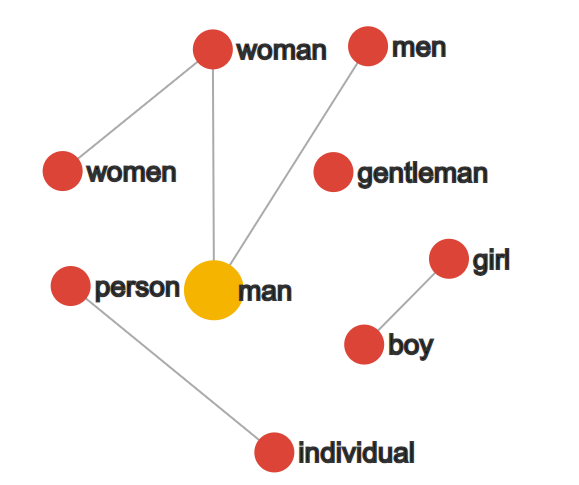
\includegraphics[width=0.5\textwidth]{content/chapter_basics/images/tokenize_transformation.png}
		\centering
		\caption{Tokenisierung einer JavaScript-Methode}
		\label{img:tokenize_transformation}
	\end{figure}
\end{center}


\subsubsection{Vorhersage}
Die dritte Hauptkomponente ist die Vorhersage, ist die wichtigste der Komponenten und wird in \cite{vaswani-2017} ausführlicher beschrieben. Diese Komponente macht den großen Teil der Modelle aus und ist dafür verantwortlich, dass sie zu groß sind. Die Wahl eines geeigneten Verfahrens hängt von der Fähigkeit ab mit großen Datenmengen umzugehen. Ziel ist immer möglichst viele Daten mit möglichst wenig Rechenaufwand zu trainieren. Die meisten der heutigen Modelle verwenden für die Vorhersage die Transformer-Architektur.\vspace{0.2cm}

Dabei kommen Mechanismen wie der Selbstaufmerksamkeitsmechanismus \textit{Self-Attention} zum Einsatz. Er verfügt über mehrere Schichten und verwendet meist Feedforward-Neuronale-Netze. Dies ermöglicht den Modellen die Eingabesequenzen parallel zu verarbeiten und die Textsequenzen in verschiedenen Kontexten zu betrachten. Die Technik verzichtet auf wiederkehrende Architektur wie die Faltung des neuronalen Netzes. Die Abbildung \ref{img:llm_transformer_model} zeigt alle Komponenten des Transformermodels und ist aus \cite{vaswani-2017} entnommen. Hierbei wird jedes Wort mit jedem anderen Wort des Satzes in Beziehung gebracht. Dadurch lernt das Modell, in dem es die Beziehungen vergleicht und die Worte werden gewichtet.\vspace{0.2cm}

Ein weiterer Mechanismus ist der zur Anwendung kommt, ist die \textit{Multi-Head Attention}.
% https://assets-8291.accso.de/downloads/202311_Masterarbeit_Bennet-Wilhelm.pdf S. 

\begin{center}
	\begin{figure}[!ht]
		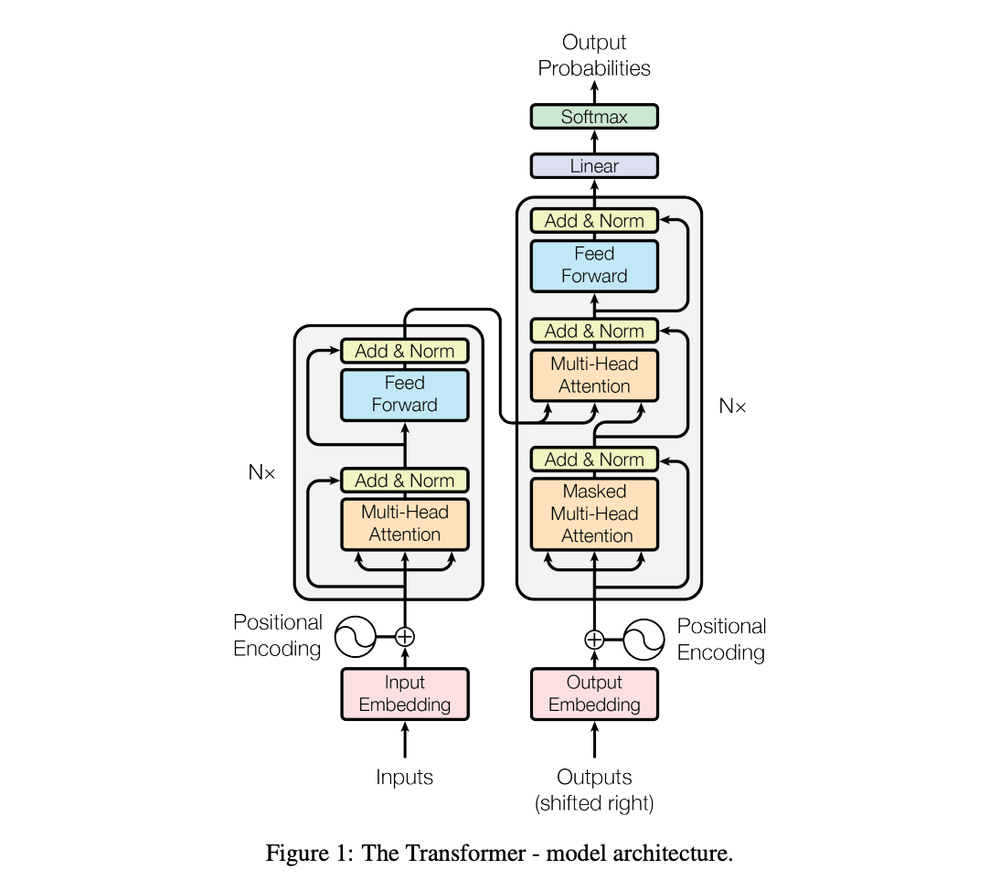
\includegraphics[width=0.8\textwidth]{content/chapter_basics/images/llm_transformer_model.png}
		\centering
		\caption{Transformermodel}
		\label{img:llm_transformer_model}
	\end{figure}
\end{center}

Der Tranformer liefert einen hochdimensionalen Vektor, der alle Informationen des Eingangstextes enthält.


\subsubsection{Dekodierung}
Dieser Vektor muss nun wieder in Text umgewandelt werden. Diese erfolgt je nach Aufgabe, um den Anforderungen gerecht zu werden. Je nach Aufgabe erfolgen dann verschiedene Verarbeitungsschritte. Beispielsweise kann bei der Textgenerierung die \glqq Greedy Decoding\grqq \ angewandt werden.\vspace{0.2cm}

Bei der Dekodierung geht es darum den wahrscheinlichsten oder eine Auswahl zutreffen aus $n$-wahrscheinlichen Token. Die Ausgaben sollen möglichst kohärente Antworten erzeugen.


\subsection{Historie der LLM}
Die Grundsteine für die Forschung der natürlichen Sprache legte Ferdinad de Saussure\footnote{Ferdinad de Saussure, lehrte von 1906 bis 1912 an der Universität Genf, Indogermanische und Allg. Sprachwissenschaften, sowie Sanskript. Er starb 1913} bereits 1906 bis 1912 an der Universität von Genf. Seine Arbeit wurde von Albert Sechehaye und Charles Bally weitergeführt und veröffentlichte in seinen Namen das Werk \glqq Grundlagen der allgemeinen Sprachwissenschaften\grqq .
%https://bop.unibe.ch/iw/article/view/11053/13941

\begin{center}
	\begin{figure}[!ht]
		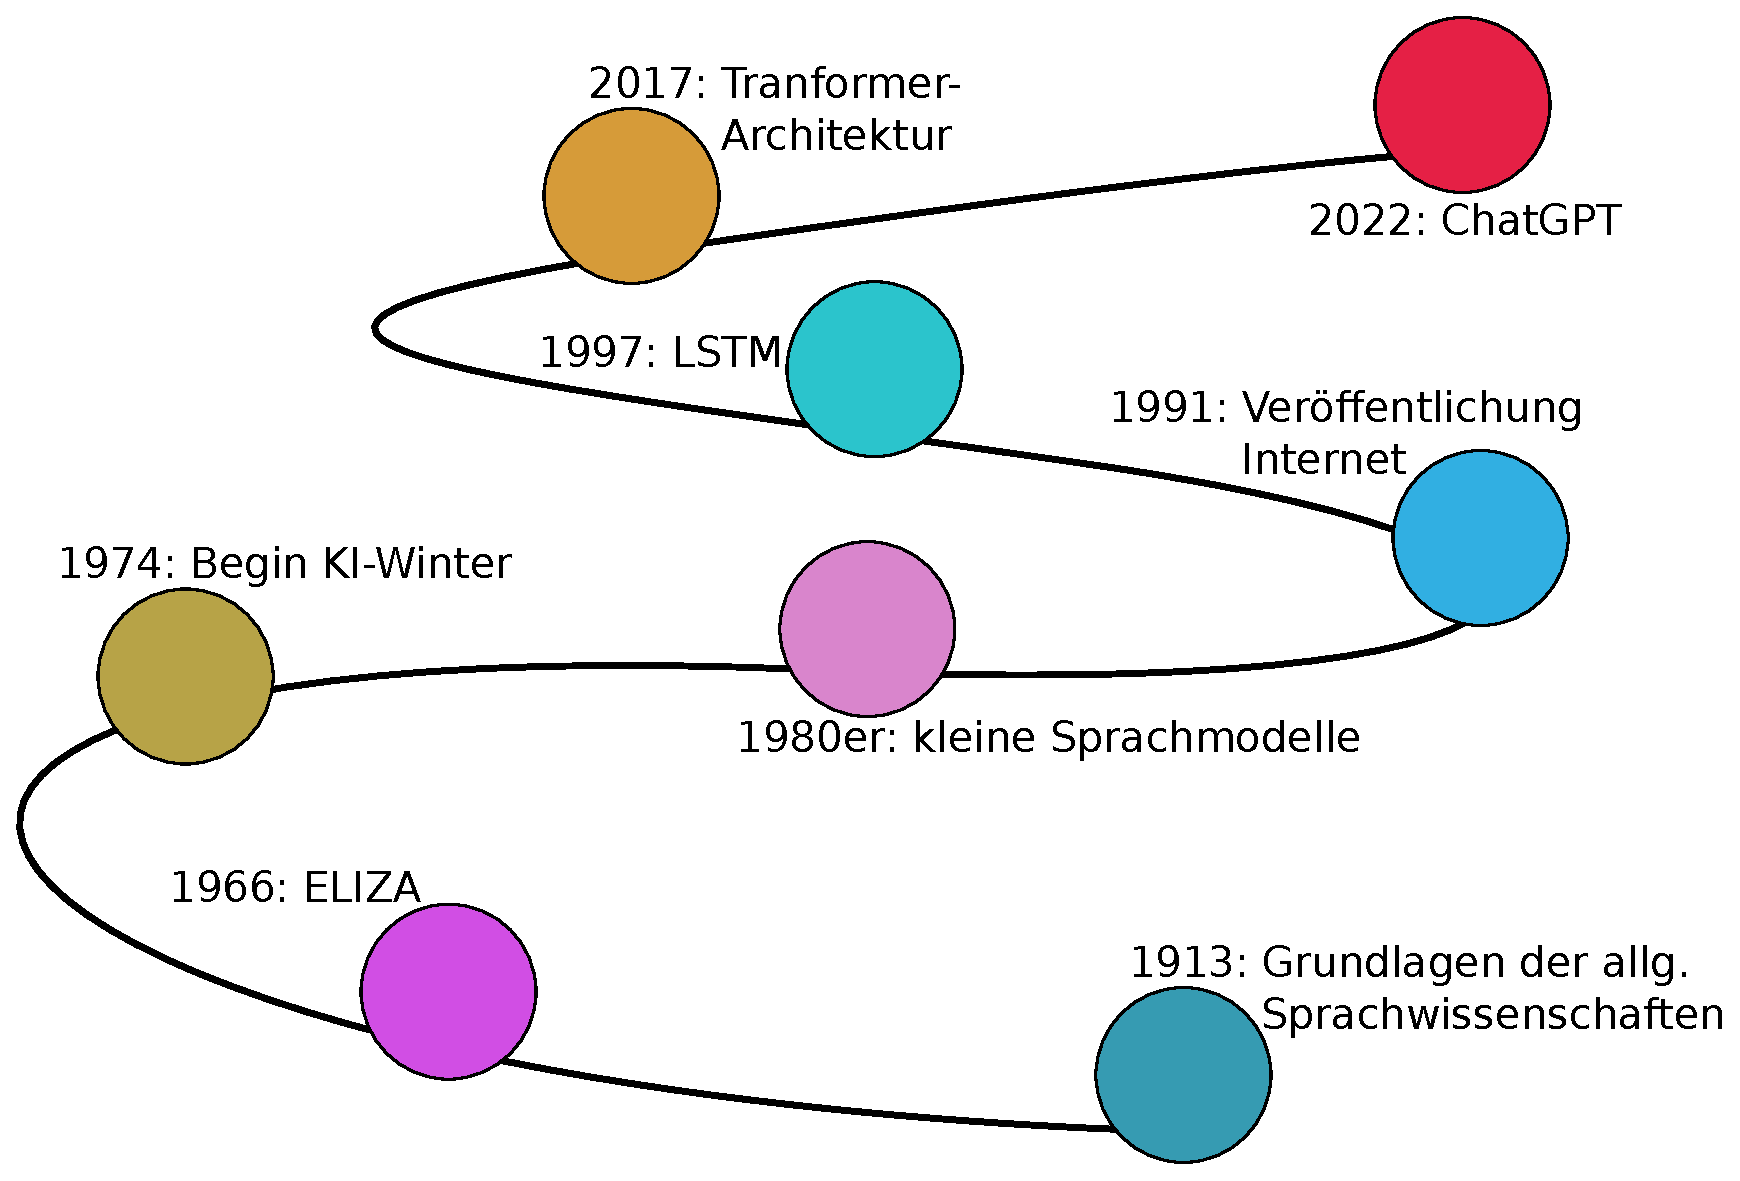
\includegraphics[width=0.8\textwidth]{content/chapter_basics/images/evolution_of_llm.eps}
		\centering
		\caption{Entwicklung der Large Language Model}
		\label{img:evolotion_of_llm}
	\end{figure}
\end{center}

Das erste Programm welches \acrshort{NLP} anwandte, war ELIZA. Es war der erste Chatbot, der im Jahr 1966 von MIT-Informatiker Joseph Weizenbaum entwickelt wurde. Das Programm verwendetet eine Mustererkennung in den Nutzereingaben und konnte so eine menschliche Konversation simulieren. Dies sollte der Beginn der Erforschung und Entwicklung natürlicher Sprache und noch besseren LLMs sein.\vspace{0.2cm}

In der Zeit von 1974 bis 1980 spricht man vom \glqq ersten KI-Winter\grqq . Viele Universitäten hatten die Forschung an neuronalen Netzen eingestellt und die Forscher organisierten sich neu und verlagerten ihren Schwerpunkt auf Wahrscheinlichkeitstheorie und Statistik. Neuronale Netze und Maschine Learning wurde hauptsächlich dafür genutzt,um Telefonanrufe zu beantworten und andere automatisierbare Prozess zu erledigen.\vspace{0.2cm}

In den 1980er wurden die ersten kleinen Sprachmodelle entwickelt. Diese Modelle wurden hauptsächlich entwickelt, um das nächste Wort in einem Satz hervorsagen zu können. Sie konnten mit kleinen Datensätzen trainiert werden und berechneten nach jedem neuen Wort das nächste Wort neu.\vspace{0.2cm}

Ende der 1980er nahm die Rechenleistung enorm zu und auch die Algorithmen bei der Verarbeitung natürlicher Sprache verbesserten sich zusehends. Hinzu kam das 1989 erfundene Internet, was 1991 der Öffentlichkeit zugänglich wurde. Damit wuchsen in den 1990er riesige Datenmengen, die für das Training der Modelle verwendet werden konnten.\vspace{0.2cm}

Ab den 1990er Jahren wurden im Bereich Deep Learning große Fortschritte erzielt und die ersten großen Sprachmodelle wurden entwickelt. Diese Modelle arbeiteten ebenfalls mit neuronalen Netzen. Im Jahr 1997 wurden Long Short-Term Memory Netzwerke eingeführt, welche tiefe und komplexe neuronale Netzwerke ermöglichten, die große Datenmengen verarbeiten konnten.\vspace{0.2cm}

Im Jahr 2017 führte Google Brain die Transfomer-Architektur ein, die bis heute in großen Sprachmodellen verwendet wird. Der große Hype um KI und den großen Sprachmodellen wurde mit der Einführung von ChatGPT, im November 2022 ausgelöst. In den Folgejahren haben Lösungen wie Hugging Face\footnote{Hugging Face, ist ein US-Unternehmen die Anwendungen für ML entwickeln und besonders für ihre Transformer-Bibliotheken bekannt sind} und BARD\footnote{BARD, ist eine von Google entwickeltes kostenlosen großes Sprachmodell, welches im März 2023 veröffentlicht wurde. Es kann über Text-, Bild- oder Audiodateien interagieren} zur Weiterentwicklung erheblich beigetragen.


\subsection{Grenzen und Probleme bei LLMs}
Sind zwar toll können aber nicht alles.

\subsubsection{Halluzinationen}
% https://www.unite.ai/de/Die-Bek%C3%A4mpfung-von-Halluzinationen-in-gro%C3%9Fen-Sprachmodellen-ist-ein-%C3%9Cberblick-%C3%BCber-modernste-Techniken/


\subsubsection{Mangel an Verständnis}
Kennen nicht die ganze Welt, nur ihre Muster von den Trainingsdaten. Ausgaben sind darauf beschränkt.


\subsubsection{Ressourcenverbrauch}
Hohe Rechenleistung für das Training, auch mal mehrere Monate.


\subsubsection{Kreativitätsbegrenzung}
Keine innovativen Ideen entwickeln.


\subsubsection{Trainingsdaten}
Shit in shit out.


\subsubsection{Transparenz}
Ergebnisse schwer nachvollziehbar.


\section{Koordinationsstrategien für LLMs}
Die Large Languarge Models haben große Leistungen auf dem Gebiet der Verarbeitung natürlicher Sprache gezeigt. Zunehmend arbeiten mehrere LLMs für diese Aufgaben zusammen. In diesem Fall spricht man von Agenten, die jeweils eine LLM darstellen können.\vspace{0.2cm}

Werden für unterschiedliche Aufgaben verschiedene Modelle verwendet, spricht man von Agenten. Ein Agent ist eine autonome Einheit. Sie ist in der Lage ihre Umwelt wahr zunehmen, Entscheidungen zu treffen und führt ihre Handlungen aus, um ein definiertes Ziel zu erreichen. Dies kann beispielsweise durch die \gls{bdi_architectur} umgesetzt werden. Jeder Agent ist auf unterschiedliche Aufgaben spezialisiert. In \cite{du-2024} werden Multi-Agenten-System mit Team aus der Softwareentwicklung verglichen und gleich gesetzt.\vspace{0.2cm}

Es gibt einige Methoden Large Language Model miteinander zu kombinieren, beispielsweise \glqq Pipeline-Architektur\grqq \ und \glqq Modular Approaches\grqq . Im Folgen Kapiteln werden die zwei Ansätze für die Zusammenarbeit von mehreren LLMs, \textit{Orchestrierung} und \textit{Multi-Agenten-System (MAS)} kurz erläutert.

\subsection{Orchestrierung von LLMs}
Bei der Orchestrierung von LLMs wird die Steuerung, der Agenten mittels eines zentralisierten Systems umgesetzt, es erfolgt eine koordinierte Nutzung. Meist wird ein Problem in Teilprobleme zerlegt und die Agenten bearbeiten Teilprobleme meist parallel. Die zentrale Steuerung entscheidet welche Teilaufgabe, welcher Agent am besten geeignet ist für die Lösung der Teilaufgabe.\vspace{0.2cm}

Die zentrale Rolle in der Orchestrierung von LLMs übernimmt dabei der Orchestrator. Dieser steuert die Aufgabenverteilung, koordiniert und kombiniert die Ergebnisse und leitet sie in die entsprechenden Agenten oder erstellt daraus die Antwort, außerdem kann er zusätzliche Aufgaben wie Fehlerbehandlung, Skalierung, Datenschutz und Sicherheit ausführen.\vspace{0.2cm}

Im Bereich der Softwareentwicklung mit Spezialisierung auf internetbasierte Anwendungen, bei der bestimmte Standards erwartet, spezielle Frameworks und Bibliotheken eingesetzt werden, könnte eine Orchestrierung bei der Umsetzung der Programmcodeerstellung wie folgt beschrieben, helfen. Bei der Lösung von Anforderungen sind nicht immer alle Agent beteiligt, vielmehr sucht der Orchestrator die jeweiligen optimalen Agenten aus.\vspace{0.2cm}

Der Orchestrator übernimmt auch hier die oben beschriebenen Aufgaben. Ein Frontend-Agent nutzt eines der großen Sprachmodelle, um Nutzeranforderungen in die Benutzeroberflächen der Anwendungen zu implementieren und könnte das Design verwalten. Gleichzeit wäre es möglich, dass dieser Agent Tools wie React.js oder Vue.js unterstützen. Für die serverseitigen Anwendungen ist der \textit{Backend-Agent} verantwortlich und verwaltet die Logik der Anwendung. Er könnte mit Frameworks wie Node.js, Express und Django umgehen. Um die Anwendung mit einer Datenbank auszustatten, kann ein \textit{Datenbank-Agent} eingesetzt werden. Er kennt verschiedenen Datenbanken wie MySQL oder PostgreSQL. Dieser verwaltet die Datenbank und deren Abfragen. Der \textit{Test-Agent} testet die Anforderung die von durch den Frontend-, Backenend- oder Datenbank-Agent umsetzt wurden.\vspace{0.2cm}

Ein letzter wichtiger Agent könnte noch der NLP-Agent sein. Dieser Agent nimmt natürliche Sprachanweisungen und Anforderungen entgegen, übersetzt diese in technische Anforderungen als Prompt für die Sprachmodelle. Die Ergebnisse der Bearbeitung werden zum Schluss von dem Agenten in eine vom Menschlichen verständliche Sprache überführt und zurückgegeben.

\subsection{Multi-Agenten-Systeme}
Multi-Agenten-Systeme (\acrshort{MAS}) bestehen ebenfalls aus mehreren Agenten. Im Gegensatz zur Orchestrierung sind Multi-Agenten-Systeme in ihrer Steuerung dezentralisiert. Alle Agenten haben unterschiedliche Lösungsansätze für ein Problem. Je nach deren Fähigkeit hat dieser auch seine ganz eigenen Ziele, welche zu den anderen Agenten entweder als \gls{collaborative} oder als \gls{competitive} ausgerichtet sind. Die Hauptarbeit zur Lösungsfindung eines Problems übernimmt der Agent, mit dem besten Lösungsansatz für das Problem. Die anderen Agenten können den ausführenden Agenten unterstützen. Um die beste Lösung zu finden, müssen die Agenten untereinander kommunizieren.  Teil der Kommunikation kann es sein, einfache Informationen austauschen, um eine gemeinsame Strategie fest zulegen oder um zu Verhandeln, welcher Agent die Lösung eines Problems übernimmt.\vspace{0.2cm}

Im Bereich der Webentwicklung mit MAS, könnte ein derartiges System wie folgt aussehen und folgende Aufgaben übernehmen. Auch hier werden nicht alle Agenten für die Lösung einer Anforderung benötigt. Vielmehr entscheidet jeder Agent für sich, ob und wie viel er zur Lösung betragen kann.

Die Abbildung \ref{img:mas_web_development_schema} zeigt das Schema eines MAS für die Webentwicklung.

\begin{center}
	\begin{figure}[!ht]
		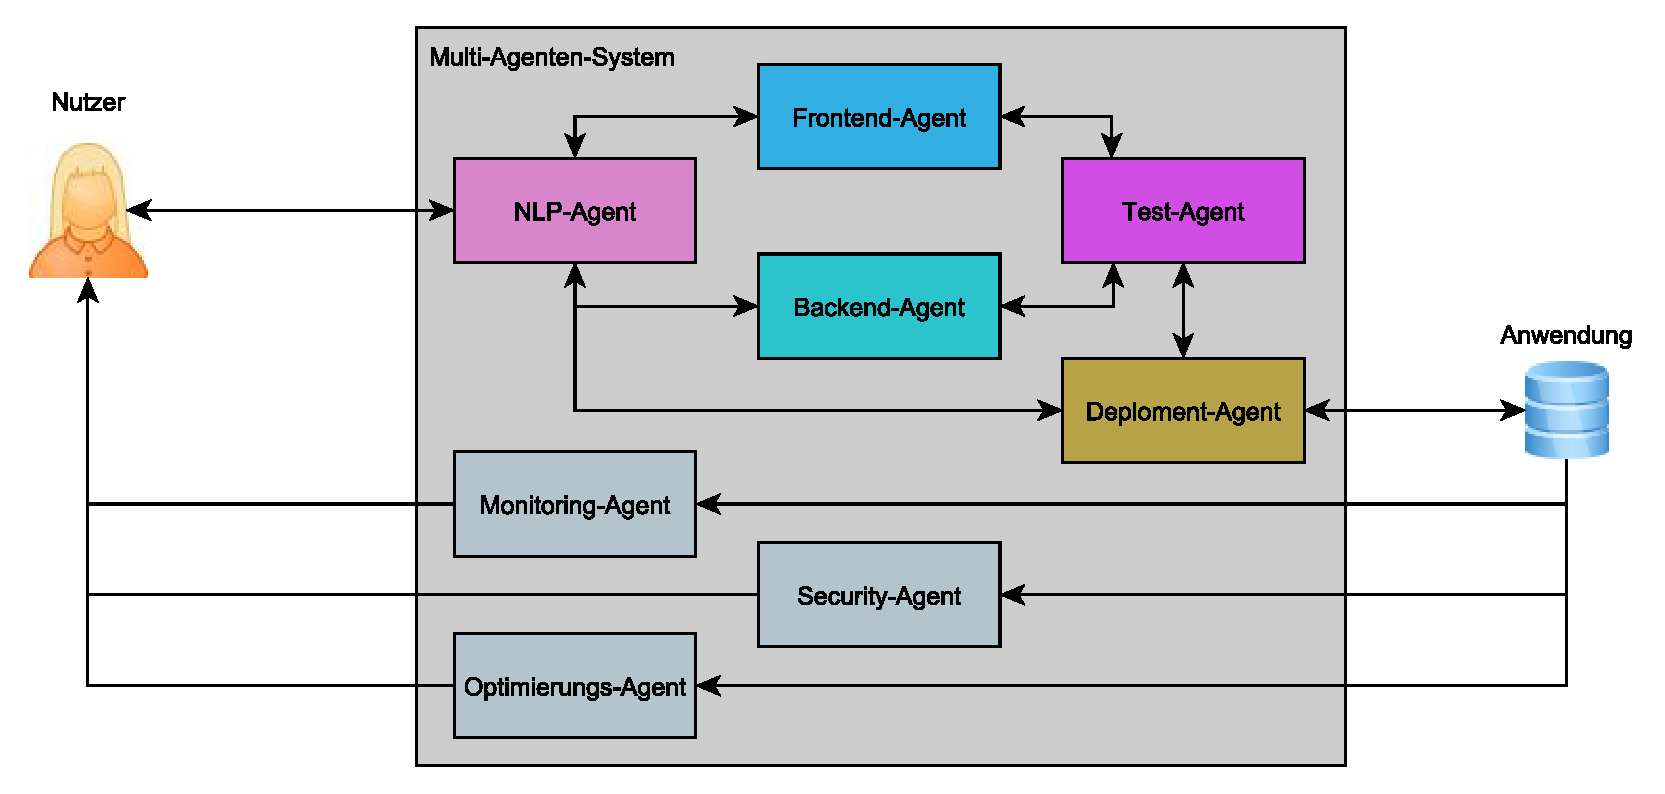
\includegraphics[width=0.8\textwidth]{content/chapter_basics/images/mas_web_development_schema.eps}
		\centering
		\caption{Multi-Agenten-System in der Webentwicklung}
		\label{img:mas_web_development_schema}
	\end{figure}
\end{center}

Ein \textit{Frontend-Agent} ist für das Design und die Benutzeroberfläche verantwortlich. Hierbei erzeugt dieser Agent Ausgaben in HTML, JavaScript und CSS um die Oberflächen zu erstellen. Dazu kann er Frameworks, wie React verwenden und auf externe Designer Tool zugreifen. Ein weiterer Agent ist der \textit{Backend-Agent}, der für die serverseitige Anwendung zuständig ist. Er erstellt seine Funktionen in PHP, Python oder NodeJS. Der Backend-Agent hat Zugriff auf Frameworks und externe Bibliotheken. Der erstellt und verwaltet zudem die Datenbankoperationen (CRUD-Operations). Hinzu kommt noch ein \textit{Test-Agent}, welcher automatisierte Tests durchführt. Um die Funktionalität der Anwendung zu gewährleisten, arbeitet der Test-Agent mit dem Frontend- und Backend-Agent eng zusammen. Der Test-Agent stellt sicher, dass jegliche Codeänderung getestet wird und führt Unit-, Inetragtions- und End-to-End-Tests durch. Wird ein Fehler festgestellt, kann der Test-Agent ein Ticket erstellen oder direkt mit dem Frontend- oder Backend-Agenten kommunizieren.\vspace{0.2cm}

Ein weiterer Agent könnte ein \textit{Deploment-Agent} sein. Dieser führt automatische Depolyments in verschiedene Umgebungen (QA, Test oder Produktion) durch. Er ist in den Continuous Integration (CI) und Continuous Deployment (CD) Workflow integriert, welche die Bereitstellung auf verschiedenen Servern (VMware, Bare-Metal) und Cloud-Umgebungen (AWS, Azure, Google) bewerkstelligt. Des weitere könnten beispielsweise Security-Agent, Monitoring-Agent und Optimierungs-Agent Einsatz finden.\vspace{0.2cm}

Auch hier kann ein NLP-Agent zum Einsatz kommen und die Kommunikation zwischen Mensch und System managen.

% https://medium.com/scisharp/understand-the-llm-agent-orchestration-043ebfaead1f

%----------------------------------------------------------------

\section{Prompt Engineering}
Prompt Engineering optimiert die Antworten große Sprachmodelle, ohne Parameter, wie Bias und Gewichte des Models ändern zu müssen. Dieser Bereich hat in den letzten Jahren enorm an Bedeutung gewonnen und sich zu einer eigenen Disziplin im Bereich der Künstlichen Intelligenz entwickelt.\vspace{0.2cm}

Ein Prompt oder Anweisung muss entweder als Anweisung oder als Frage gestellt werden. Dies kann, wie in \cite{amatriain-2024} beschrieben, in Form von einer einfachen Anweisung bis hin zu detaillierten Beschreibungen oder spezifischen Aufgaben erfolgen.\vspace{0.2cm}

[Hier Beispiel von ChatGPT oder Gemini einfügen, kann als Bild]


\subsection{Prompt-Techniken}
Siehe Prompting Techniques Hinweise für die Optimierung von Prompts.
Die folgenden Techniken dienen dazu die Abfragen zu optimieren und somit eine bessere Antwort von den Sprachmodellen zu erhalten.


\subsubsection{Zero-shot Prompting}
Bei dieser Technik handelt es sich um das Senden einer einfache, klare und präzise Anweisungen, ohne Angabe von Beispielen und sonstigen zusätzlichen Informationen an die Modelle. Hierbei handelt es sich meistens um eine Domain-spezifische Anweisung. Es findet kein explizites Training vorher statt. Die Anweisung sollte ein klar definiertes Ziel haben\vspace{0.2cm}

\lstinputlisting[label={code:prompt_zero_shot},caption={Zero-Shot Prompt als Python-String},language=Python]{content/chapter_basics/codes/zero-shot-prompt-string.py}

Im Folgenden die Antwort vom Modell. Hierbei wurde das Modell \textit{deepseek-coder-v2} verwendet und über die API abgefragt.

\lstinputlisting[label={code:answer_zero_shot_prompt},caption={Antwort des Zero-Shot-Prompts},language=text]{content/chapter_basics/codes/answer-zero-shot-prompt.md}

Um bessere Lösungen von den Modellen zu bekommen, kann es sinnvoll sein, weitere Angaben, zum Beispiel zur Arbeitsweise oder die Definition, der zu verwendenden Bibliotheken hinzuzufügen. In \cite{wei-2021} wird eine Methode vorgeschlagen, zur Verbesserung der Zero-shot Anweisungen.


\subsubsection{Few-Shot Prompting}
Bei komplexen Aufgaben liefert die Verwendung von Zero-shot Anweisungen oft unzureichende Ergebnisse. Hierfür finden Few-shot Prompts Verwendung. Bei dieser Technik werden ein oder mehrere Beispiele einer Antwort der Anweisung beigefügt, die als eine Art Antwortvorlage für das Modell dienen. Das Listings \ref{code:few-shot-prompt-as-python-string} zeigt beispielhaft den Prompt als Python-String, welcher an das Modell übertragen wurde.\vspace{0.2cm}


\lstinputlisting[label={code:prompt_few_shot},caption={Few-Shot Prompt als Python-String},language=Python]{content/chapter_basics/codes/few-shot-prompt-string.py}

Das Ergebnis vom Modell \textit{deepseek-coder-va:latest} ist in Listing \ref{code:answer_few_shot_prompt} zu sehen.

\lstinputlisting[label={code:answer_few_shot_prompt},caption={Antwort des Few-Shot-Prompts},language=text]{content/chapter_basics/codes/answer-few-shot-promt.md}

Wie erfolgreich diese Technik ist, wird in \cite{brown-2020} beschrieben. Wie wichtig bei der Formulierung der Anweisungen das Format und die Beschriftung ist, zeigt \cite{min-2022} in seiner Studie. Wird ein Beispiel angegeben, kann dazu kommen, dass das Modell nicht die richtige Antwort findet. Dann sollten mehrere Beispiele an das Modell übergeben werden.


\subsubsection{Chain-of-Thought Prompting (CoT)}
Wenn mit den Zero-shot und Few-shot Techniken nicht das gewünschte Ergebnis von den Modellen erzielt wird, könnte die Chain-of-Thought \acrshort{CoT} Technik Verwendung finden. Bei dieser Technik wird das Modell aufgefordert, sein Vorgehen zu belegen. Mit dieser Technik kann besser nachvollzogen werden, wie im Modell der Lösungsversuch abläuft.\vspace{0.2cm}

\lstinputlisting[label={code:prompt_cot},caption={CoT Prompt als Python-String},language=Python]{content/chapter_basics/codes/cot-prompt-string.py}

Die Antwort.

\lstinputlisting[label={code:answer_cot_prompt},caption={Antwort des CoT-Prompts},language=text]{content/chapter_basics/codes/answer-cot-promt.md}

Wie gut die Technik bei Modellen funktioniert, wird in \cite{wei-2022} untersucht.


\subsubsection{Meta Prompting}
Für Meta Prompting, sind nach \cite{zhang-2023} die wichtigsten Merkmale wie folgt,

\begin{itemize}
	\item \textit{Strukturierung} der Prompts beispielsweise bestimmen der Denkweise oder Reihenfolge vorgeben.
	\item \textit{Syntax fokussiert}, dadurch wird die Syntax als Leitvorlage für die erwartete Antwort verwendet.
	\item \textit{abstrakte Beispiele} die sich mit der Struktur des Prompt befassen, nicht mit der expliziten Lösung, wie die inhaltsgesteuert Few-Shot-Prompts.
	\item \textit{vielseitig} lässt es zu, das der Prompt in vielen Bereichen anwendbar ist und geben Antwort auf eine Vielzahl von Problemen, sodass der Prompt nicht jedes Mal neu geschrieben werden muss.
	\item \textit{kategorischer Ansatz} strukturiert den Aufbau der Prompts in logische Anordnung und Kategorisierung 
\end{itemize}

Dem Modell wird wie bei der CoT Technik angewiesen, sein Vorgehen offen zulegen. Neben dem Ergebnis, wie beim CoT, soll hierbei auch der Ablauf und die Planung der Ergebnisfindung dargestellt werden. Ein Beispiel einer Anweisung könnte folgendermaßen aussehen und wird in Listing \ref{code:prompt_meta} gezeigt.

\lstinputlisting[label={code:prompt_meta},caption={Meta Prompt als Python-String},language=Python]{content/chapter_basics/codes/meta-prompt-string.py}

Das Listing \ref{code:answer_meta_prompt} zeigt die ausführliche Antwort. Ebenfalls wurde hier das \textit{deepseek-code-v2:latest} Modell angewandt.

\lstinputlisting[label={code:answer_meta_prompt},caption={Antwort des Meta-Prompts},language=text]{content/chapter_basics/codes/answer-meta-promt.md}

Meta-Prompts sind Token-Effizient und verringern die benötigte Anzahl an Token, da der Schwerpunkt wie beschrieben auf der Struktur liegt, nicht auf den expliziten Inhalt.


\subsubsection{Prompt Chaining}
Hierbei wird eine komplexe Aufgabe in Unteraufgaben zerlegt. Die Antwort einer Unteraufgabe dient als Eingabe für die nächste Unteraufgabe. Diese Zerlegung ist hilfreich, um Komplexität einer Aufgabe zu verringern und eine Überforderung der Modelle zu verhindern. Durch diese Technik ist eine schrittweise Näherung an die Gesamtlösung der Aufgabe möglich.\vspace{0.2cm}

Im Beispiel soll das Sprachmodell wieder eine PHP Funktion schreiben, die eine HTML Zeichenkette als PDF speichert.


\lstinputlisting[label={code:prompt_chain_1},caption={Chain Prompt Nr. 1 als Python-String},language=Python]{content/chapter_basics/codes/chain-prompt-string-1.py}

\lstinputlisting[label={code:answer_chain_1_prompt},caption={Antwort des Chain-1-Prompts},language=text]{content/chapter_basics/codes/answer-chain-prompt-1.md}


\lstinputlisting[label={code:prompt_chain_2},caption={Chain Prompt Nr. 2 als Python-String},language=Python]{content/chapter_basics/codes/chain-prompt-string-2.py}

\lstinputlisting[label={code:answer_chain_2_prompt},caption={Antwort des Chain-2-Prompts},language=text]{content/chapter_basics/codes/answer-chain-prompt-2.md}


\lstinputlisting[label={code:prompt_chain_3},caption={Chain Prompt Nr. 3 als Python-String},language=Python]{content/chapter_basics/codes/chain-prompt-string-3.py}

\lstinputlisting[label={code:answer_chain_3_prompt},caption={Antwort des Chain-3-Prompts},language=text]{content/chapter_basics/codes/answer-chain-prompt-3.md}


\subsubsection{Tree of Thoughts (ToT)}
%https://www.promptingguide.ai/techniques/tot
Diese Technik wurde von \cite{long-2023} und \cite{yao-2023} vorgeschlagen. (\acrshort{ToT}) kommt bei komplexen Anforderungen zum Einsatz, wenn einfache Techniken, die zuvor genannt wurden, nicht mehr ausreichen. Auch bei dieser Technik wird die Anforderung in keine Aufgaben zerlegt. Dann werden mehrere Lösungen pro Aufgabe erstellt und im Anschluss bewertet. Dabei entsteht eine Baustruktur, von der die besten Lösungen ausgesucht werden.

\begin{figure}[!ht]
	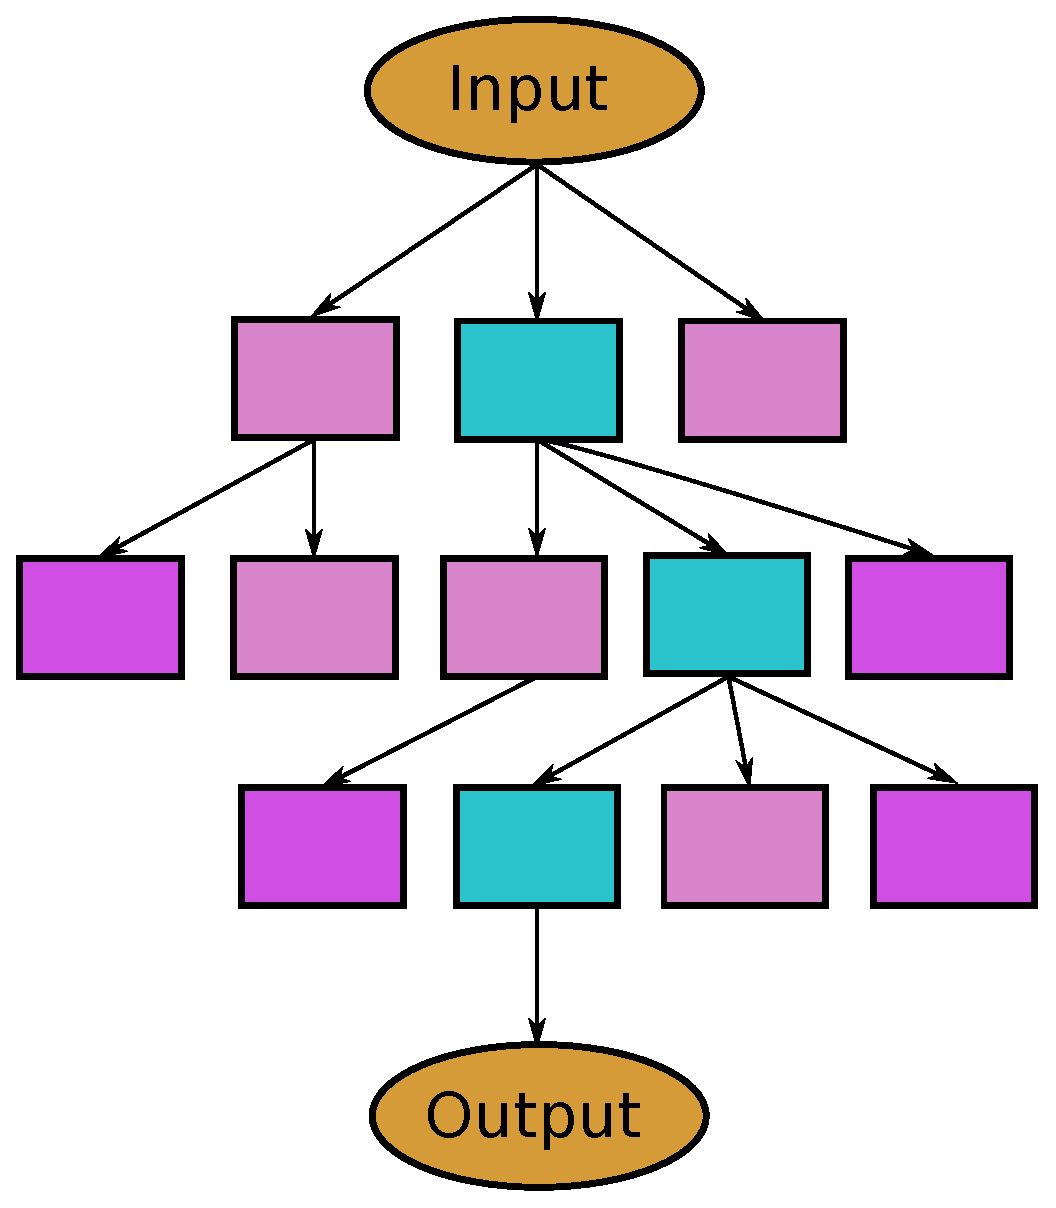
\includegraphics[width=0.4\textwidth]{content/chapter_basics/images/tot_schema.eps}
	\centering
	\caption{Baumstruktur der \glqq Tree of Thoughts\grqq \ Technik}
	\label{img:tot_schema}
\end{figure}

Im Folgenden ein Beispiel einer Teilaufgabe, bei der drei mögliche Lösungsvorschläge vom Modell erstellt wurden. Die Listings \ref{code:tot_php_dompdf}, \ref{code:tot_php_mpdf} und \ref{code:tot_php_tcpdf} zeigen die Ergebnisse des Modells. Es wurden jeweils andere PHP Bibliotheken für die Lösung vorgeschlagen. Als Modell wurde \textit{deepseek-coder-v2} verwendet. Als Nutzereingabe wurde folgendes an das Modell übergeben,

\epigraph{Erstelle drei verschiedene Methoden in PHP, die eine HTML Zeichenkette in ein PDF umwandeln und es als Datei, mit angegebenen Namen speichern.}

Die erste Lösung beinhaltet die Bibliothek \textit{Dompdf}.

\lstinputlisting[label={code:tot_php_dompdf},caption={Ausgabe für DOMPDF Bibliothek},language=PHP]{content/chapter_basics/codes/dompdf.php}

\lstinputlisting[label={code:tot_php_mpdf},caption={Ausgabe für MPDF Bibliothek},language=PHP]{content/chapter_basics/codes/mpdf.php}

Als dritte Ausgabe liefert coder,

\lstinputlisting[label={code:tot_php_tcpdf},caption={Ausgabe für TCPDF Bibliothek},language=PHP]{content/chapter_basics/codes/tcpdf.php}

%\subsubsection{Retrieval Augmented Generation}

%\subsubsection{Automatic Prompt Engineer}

%\subsubsection{Directional Stimulus Prompting}

%\subsubsection{ReAct}

%\subsubsection{Multimodal CoT}

%\subsubsection{Automatic Reasoning and Tool-use}

%\subsubsection{Active-Prompt}

%\subsubsection{Program-Aided Language Models}

%\subsubsection{Reflexion}

%\subsubsection{Graph Prompting}


\subsection{Grenzen beim Prompt-Engineering für LLMs}
Trotz der bemerkenswerten linguistischen Leistung, stoßen große Sprachmodelle an ihre Grenzen, unter anderem wie in \cite{amatriain-2024} beschrieben,

%\section{Relevante Arbeiten}
%In \cite{zhou-2022} wird der Prompt-Optimierungsprozess als Black-Box interpretiert. Der mit minimalen Eingaben ein menschenähnliches Niveau erreichen soll.

%----------------------------------------------------------------


\section{Grundlagen bei der Entwicklung von Webanwendungen}
Webanwendung
